%%%%%%%%%%%%%%%%%%%%%%%%%%%%%%%%%%%%%%%%%%%%%%%%%%%%%%%%%%%%%%%%%%%%%%%%%%%%%%%%%%%%%%%%%%%%%%%%%%%%%%%%%%%%%%%%%%%%%%%%%%%%%%%%%%%%%%%%%%%%%%%%%%%%%%%%%%%
% This is just an example/guide for you to refer to when producing your supplementary material for your Frontiers article.                                 %
%%%%%%%%%%%%%%%%%%%%%%%%%%%%%%%%%%%%%%%%%%%%%%%%%%%%%%%%%%%%%%%%%%%%%%%%%%%%%%%%%%%%%%%%%%%%%%%%%%%%%%%%%%%%%%%%%%%%%%%%%%%%%%%%%%%%%%%%%%%%%%%%%%%%%%%%%%%

%%% Version 2.5 Generated 2018/06/15 %%%
%%% You will need to have the following packages installed: datetime, fmtcount, etoolbox, fcprefix, which are normally inlcuded in WinEdt. %%%
%%% In http://www.ctan.org/ you can find the packages and how to install them, if necessary. %%%
%%%  NB logo1.jpg is required in the path in order to correctly compile front page header %%%

%\documentclass[utf8]{frontiers_suppmat} % for all articles
%\usepackage{url,hyperref,lineno,microtype}
%\usepackage[onehalfspacing]{setspace}



% Leave a blank line between paragraphs instead of using \\

%\begin{document}
%\onecolumn
%\firstpage{1}

%\title {{\helveticaitalic{Supplementary Material}}}


%\maketitle

%\section{Supplementary Tables and Figures}

\section{Figures}

\begin{figure}[htbp]
\begin{center}
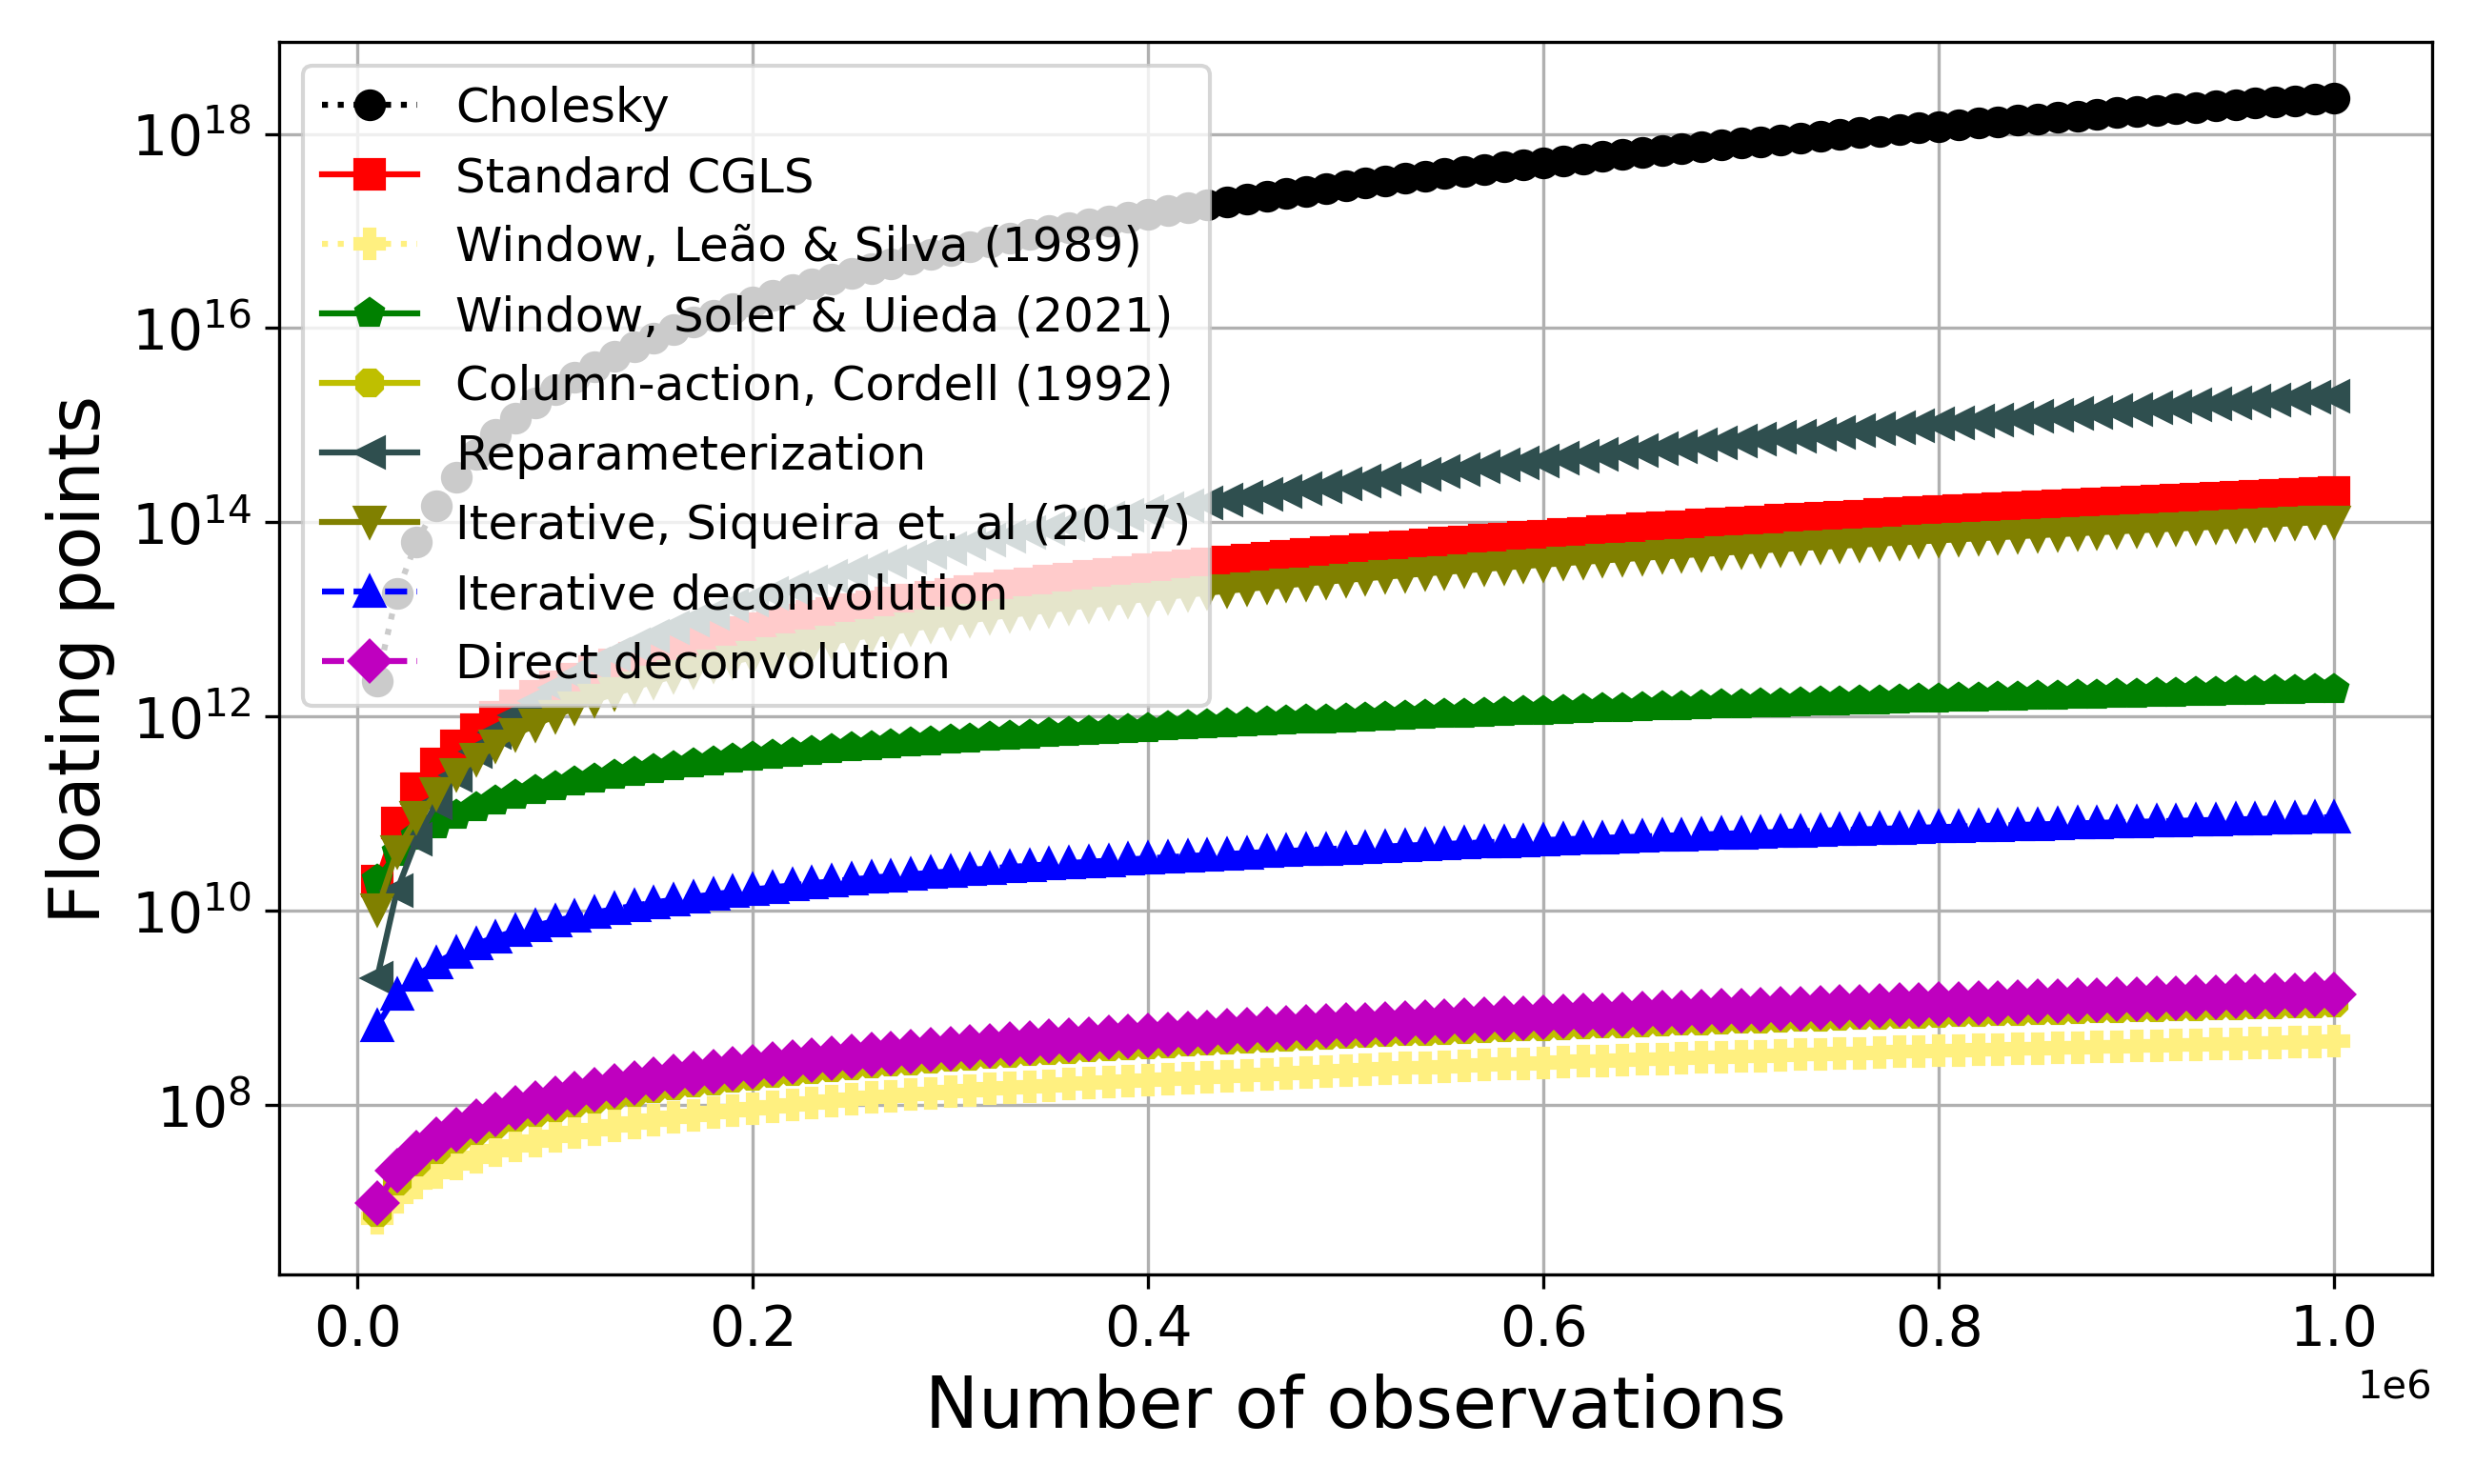
\includegraphics[width=9cm]{Fig/flops_grav}% This is a *.eps file
\end{center}
\caption{
	Total number of flops for different equivalent-layer methods
	(equations \ref{flops:cholesky}, \ref{flops:cgls}, \ref{flops:LS89}, \ref{flops:SU21}, 
	\ref{flops:C92}, \ref{flops:reparameterization-cgls}, \ref{flops:SOB17}, \ref{flops:TOB20},
	and \ref{flops:direct-deconv}). 
	The number of potential-field data $D$ varies from $10,000$ to $1,000,000$.
	}
\label{fig:1}
\end{figure}

%\begin{figure}[htbp]
%	\begin{center}
%		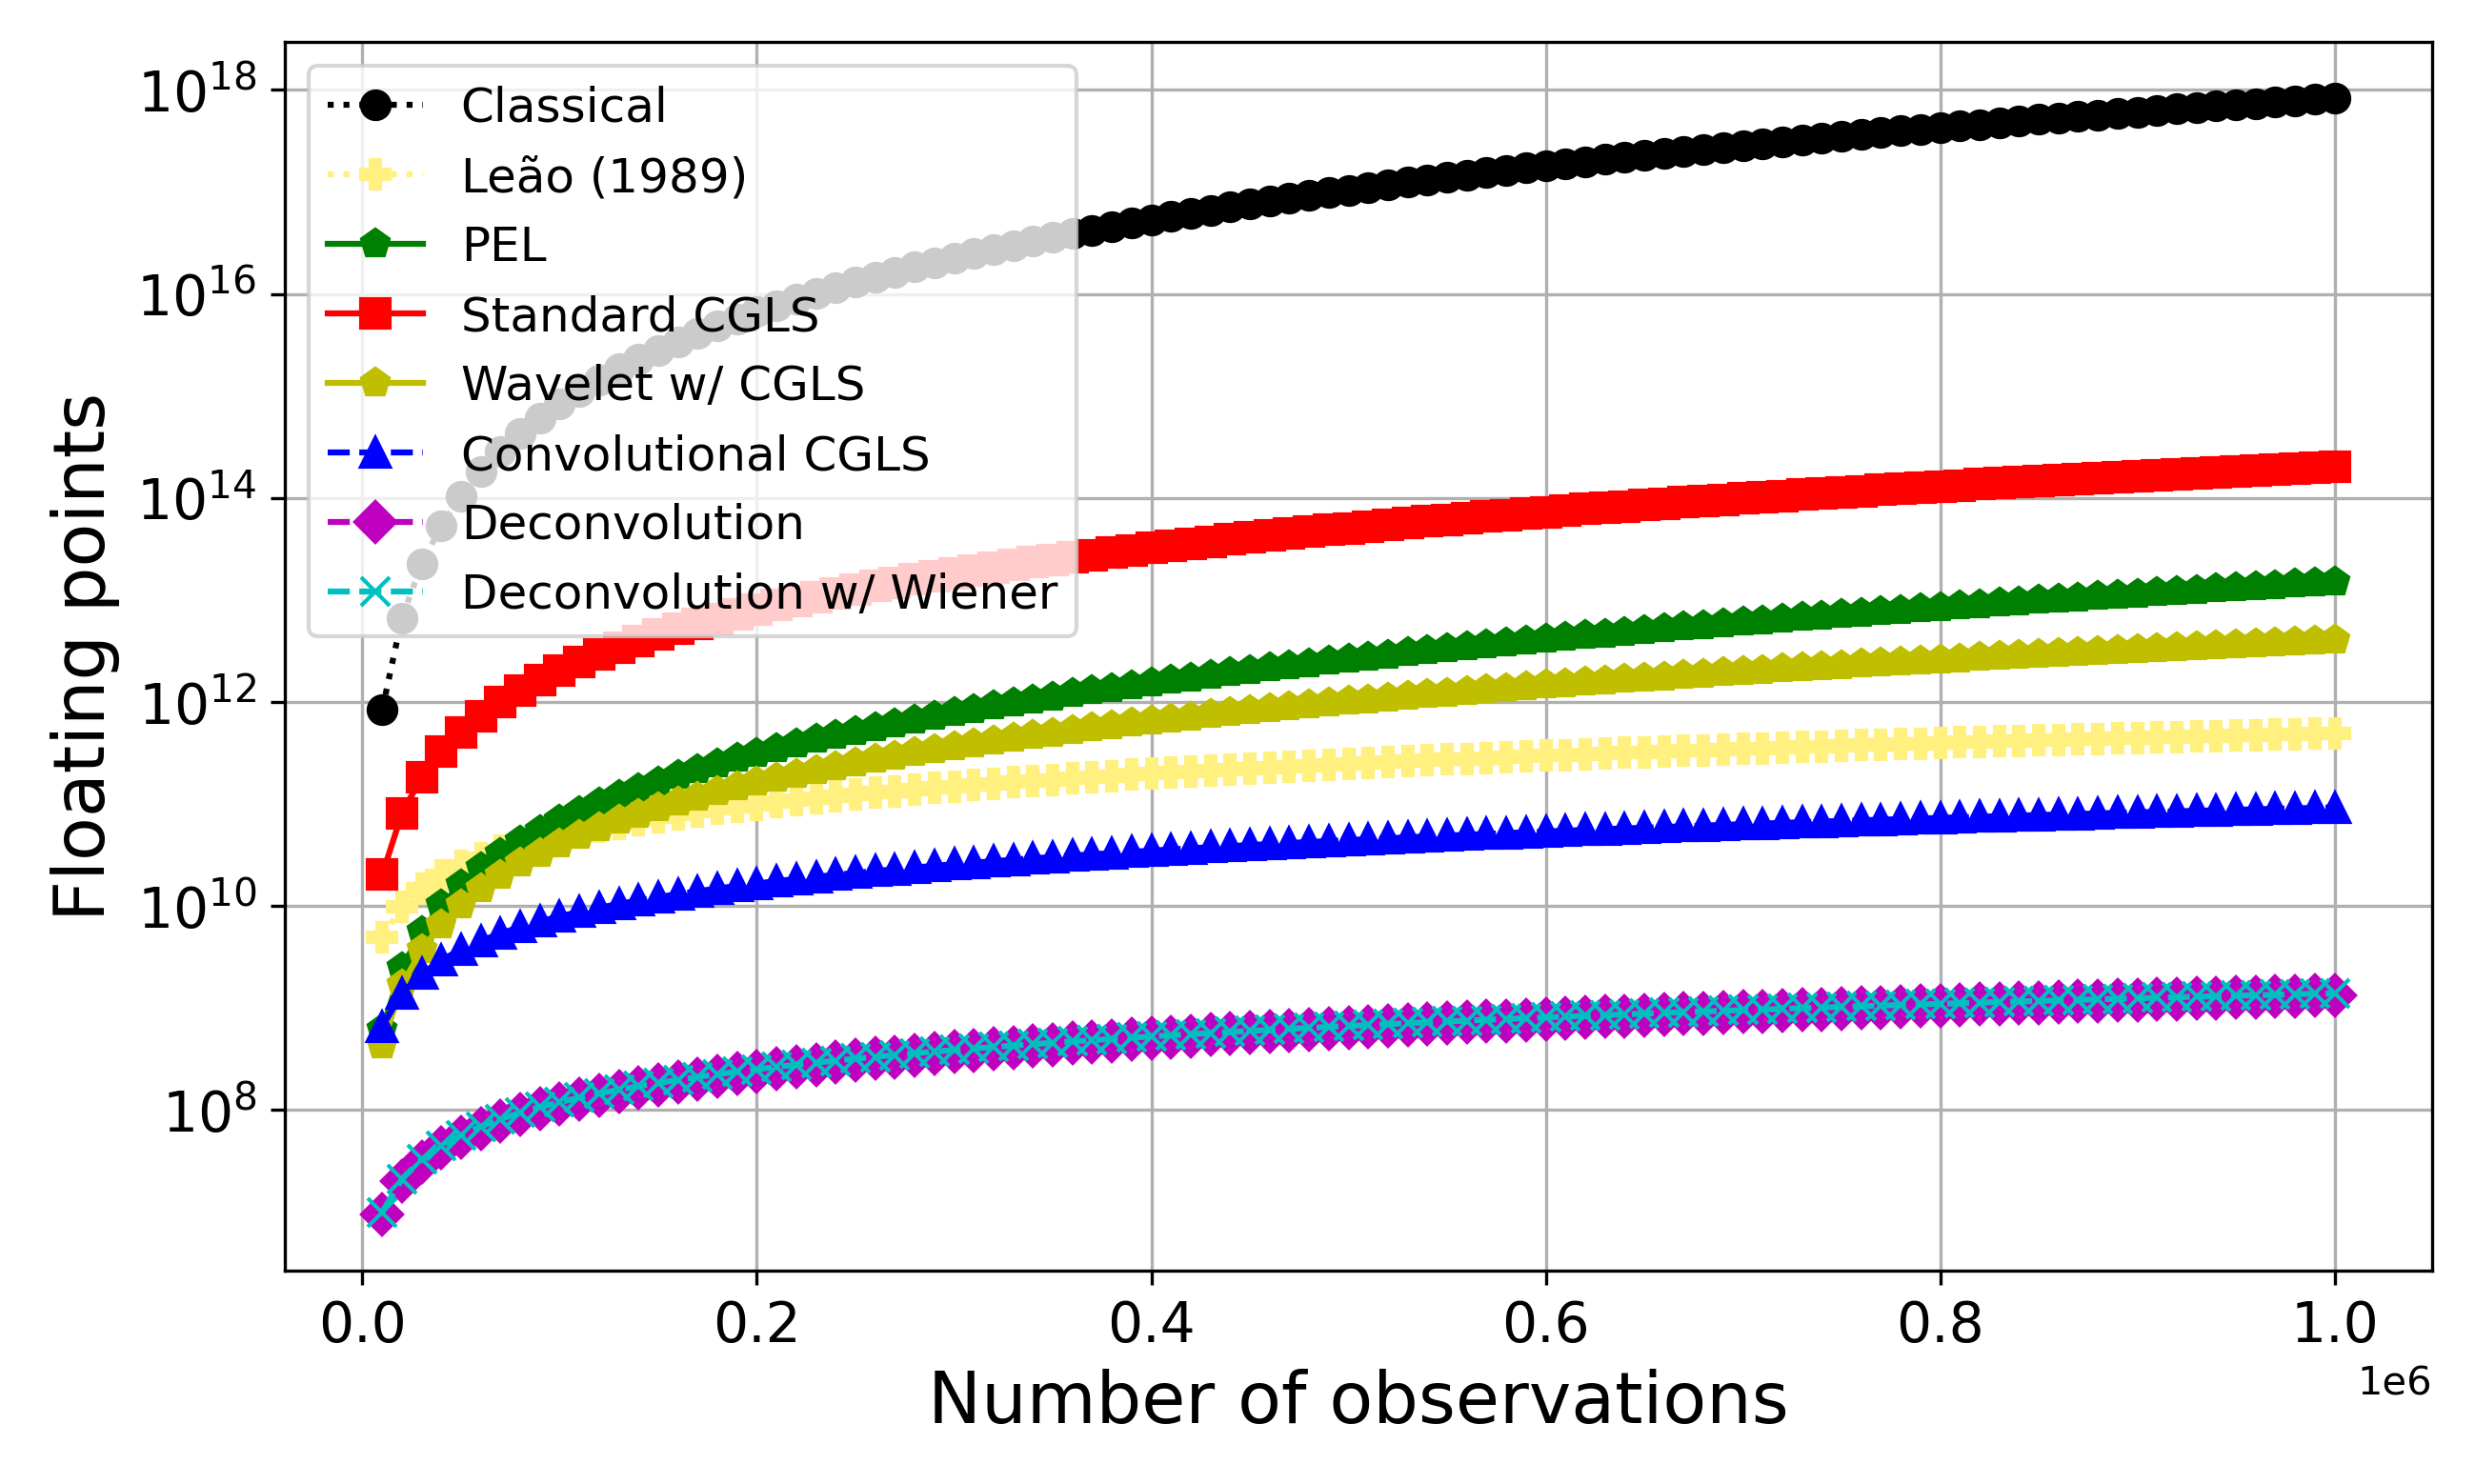
\includegraphics[width=9cm]{Fig/flops_mag}% This is a *.eps file
%	\end{center}
%	\caption{Number of \textit{flops} for many of the methods described in this work to estimate the equivalent sources using magnetic data. The range of observations varies from $10,000$ to $1,000,000$.}
%	\label{fig:2}
%\end{figure}

\begin{figure}[htbp]
	\begin{center}
			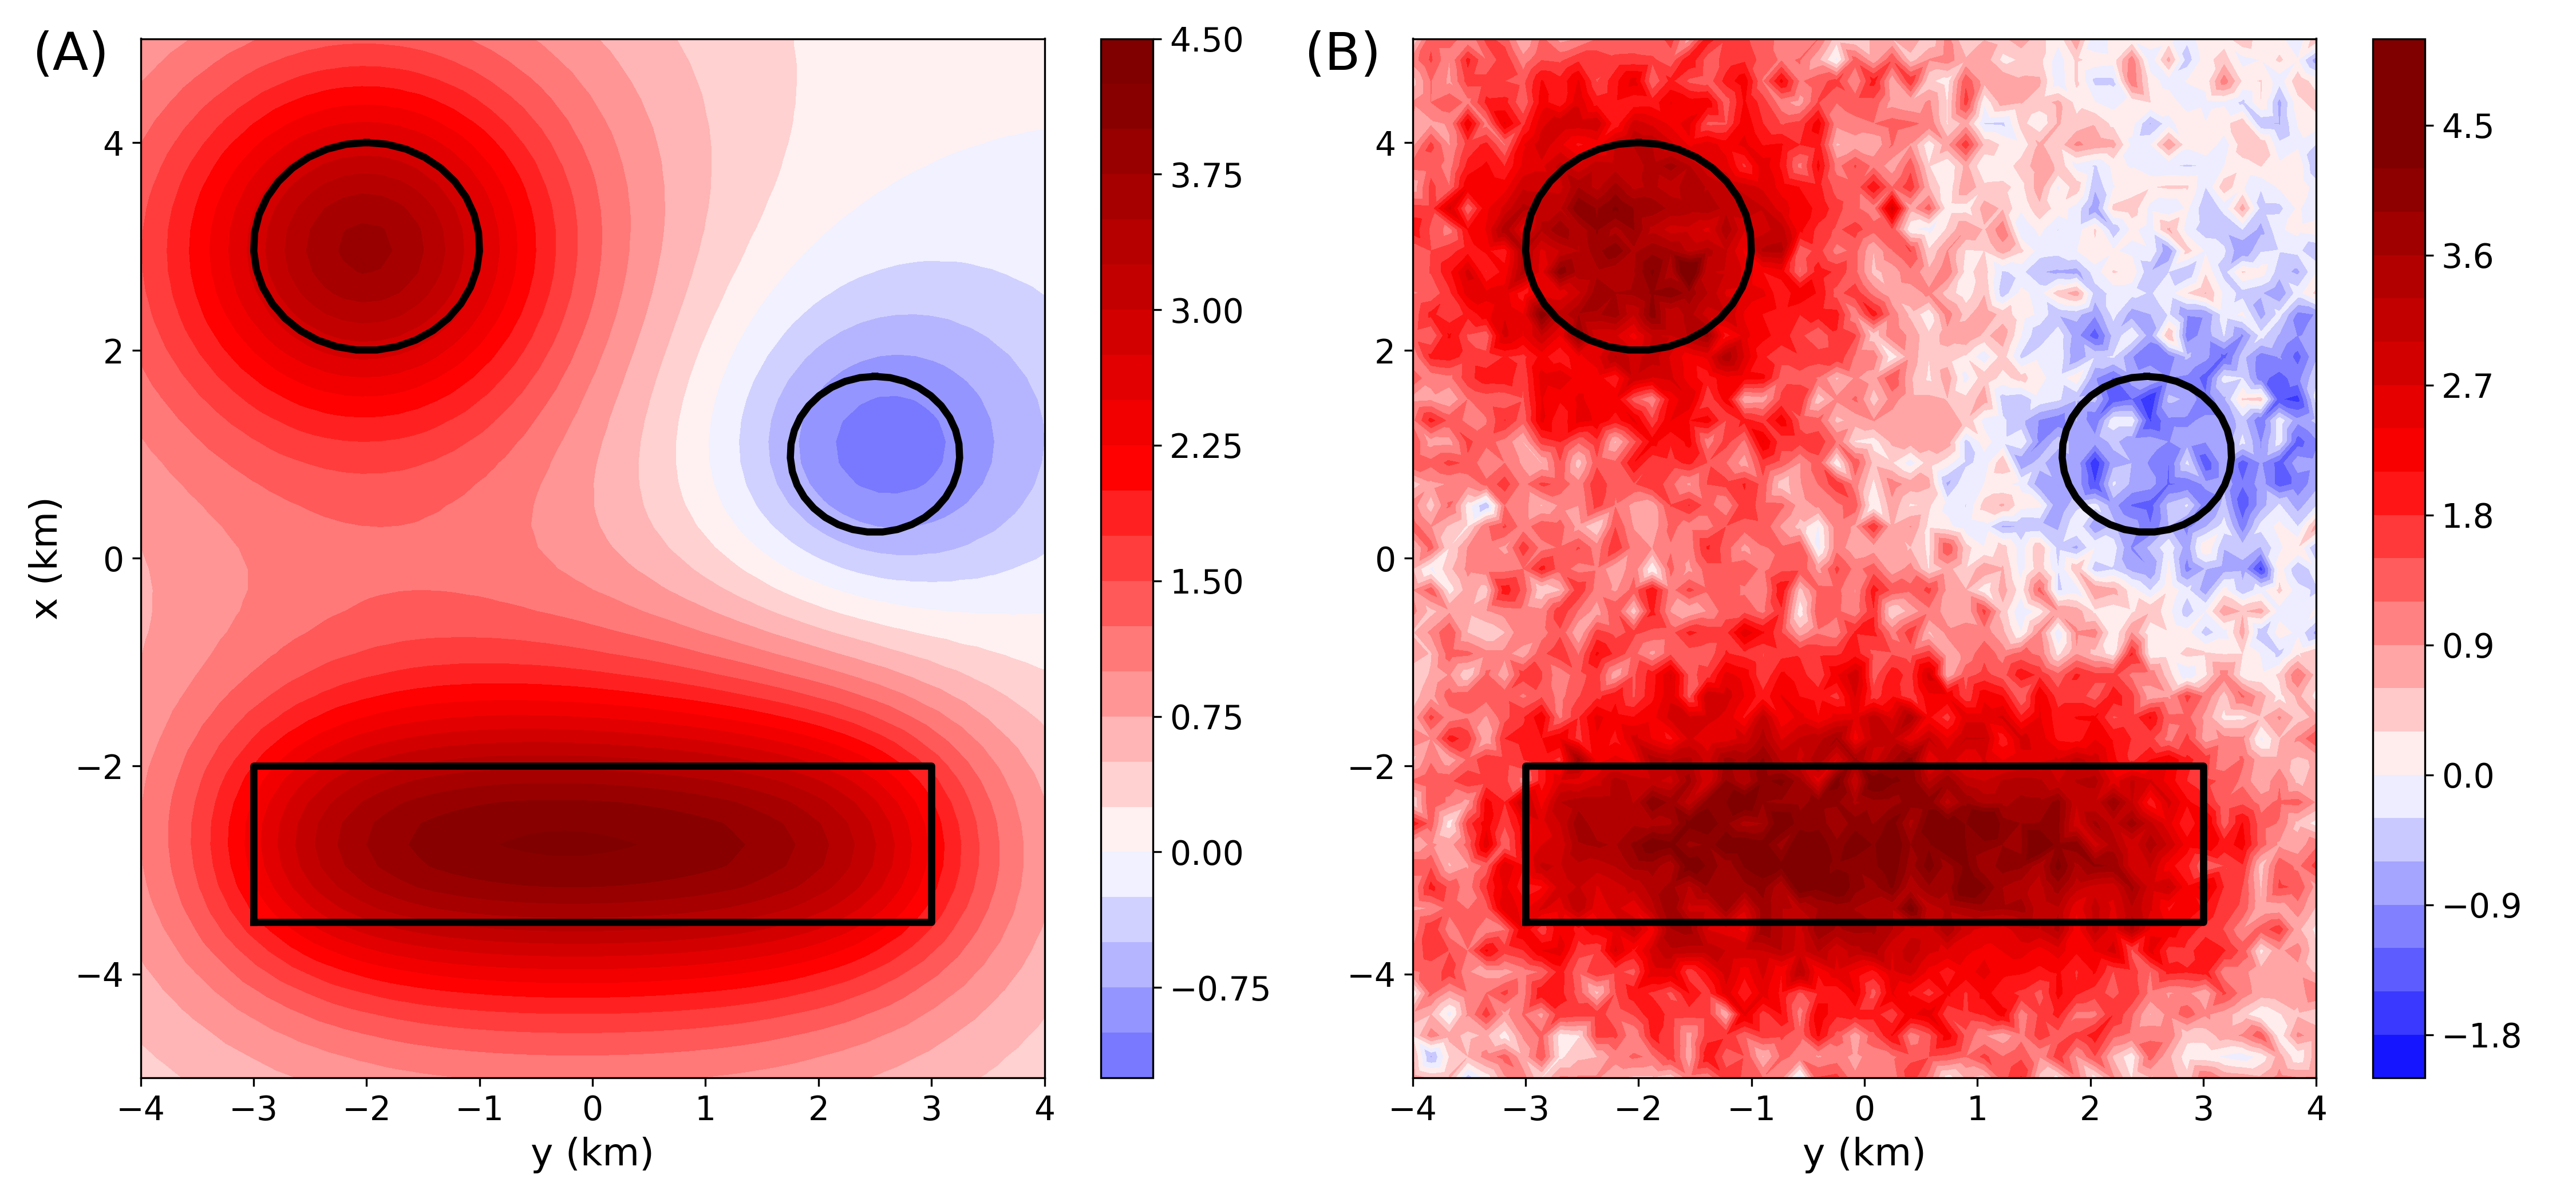
\includegraphics[width=9cm]{Fig/synthetic_grav}
		\end{center}
	\caption{
		Synthetic gravity disturbance data (in $\mathrm{mGal}$). 
		The data are located on a regular grid of $50 \times 50$ points. 
		Panel (A) shows the noise-free data. Panel (B) shows the synthetic data corrupted 
		with a pseudorandom Gaussian noise having zero mean and standard deviation equal to $10\%$
		of the maximum absolute value in the noise-free data.
		The black lines represent the projection of the synthetic bodies on the $xy$ plane.
		}
	\label{fig:4}
\end{figure}

\begin{figure}[htbp]
	\begin{center}
			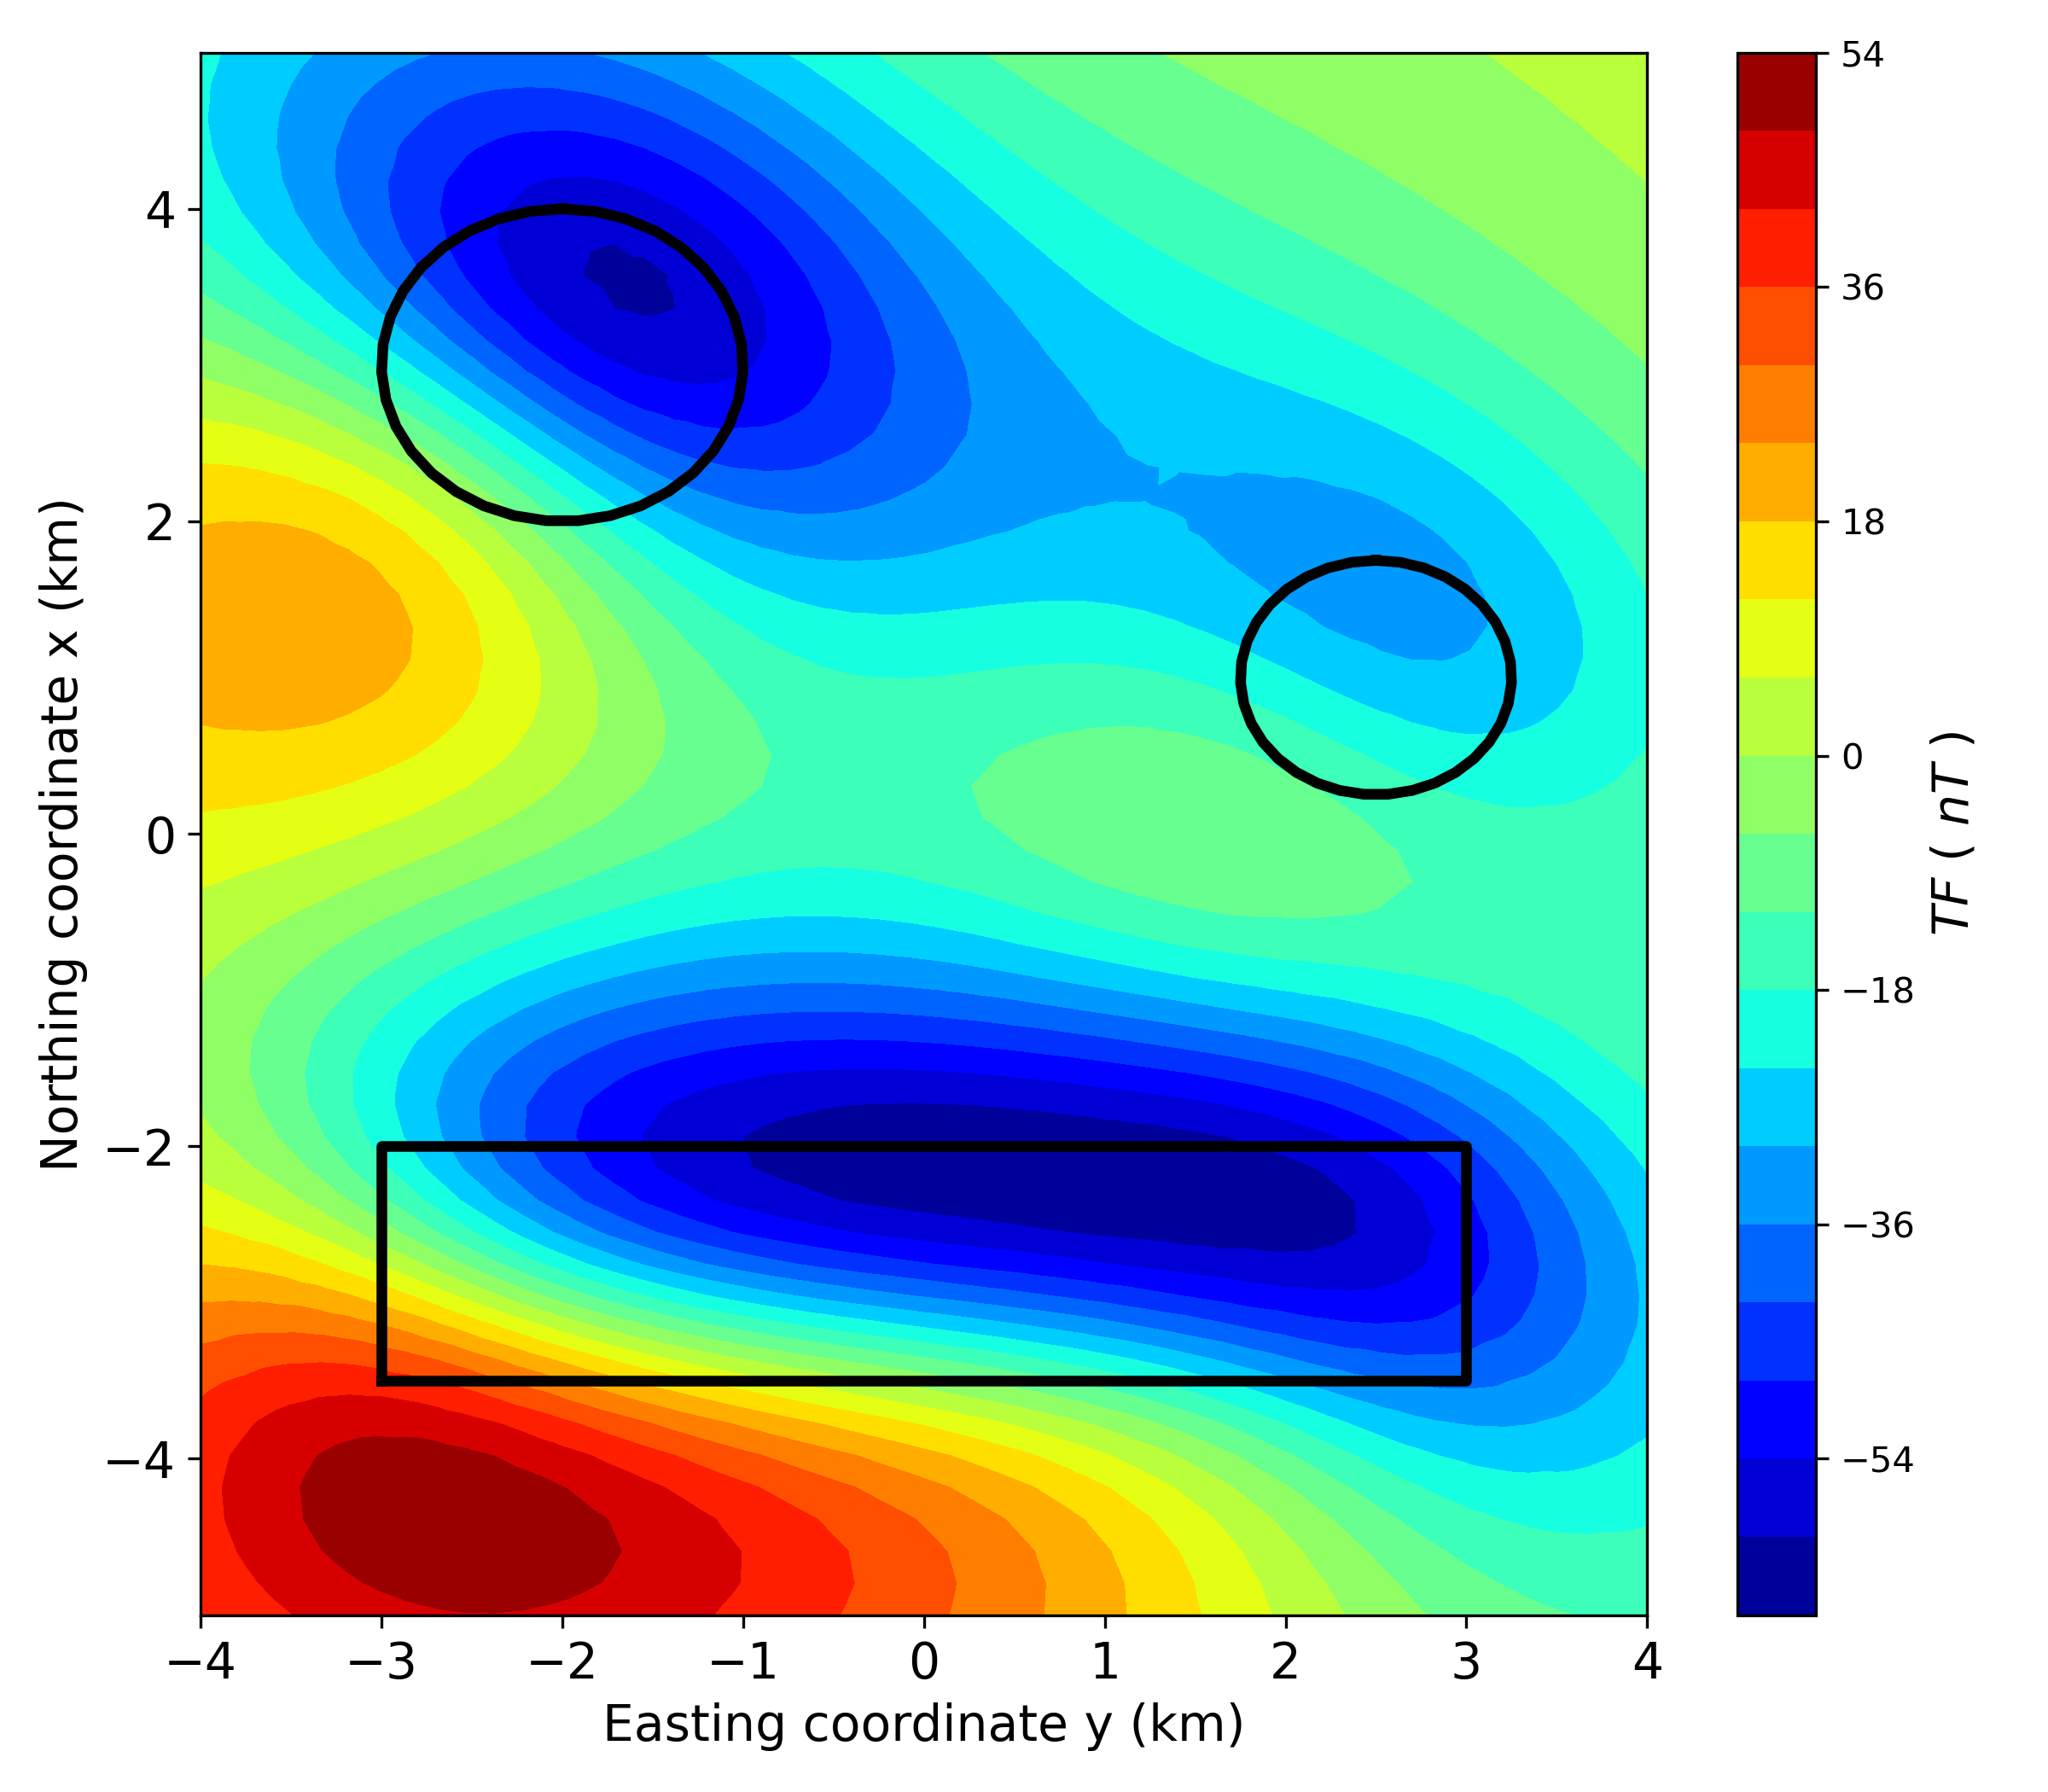
\includegraphics[width=10cm]{Fig/synthetic_mag}
		\end{center}
	\caption{
		Synthetic total-field anomaly data (in $\mathrm{nT}$). 
		The data are located on a regular grid of $50 \times 50$ points. 
		Panel (A) shows the noise-free data. Panel (B) shows the synthetic data corrupted 
		with a pseudorandom Gaussian noise having zero mean and standard deviation equal to $10\%$
		of the maximum absolute value in the noise-free data.
		The black lines represent the projection of the synthetic bodies on the $xy$ plane.
		}
	\label{fig:7}
\end{figure}

\begin{figure}[htbp]
	\begin{center}
		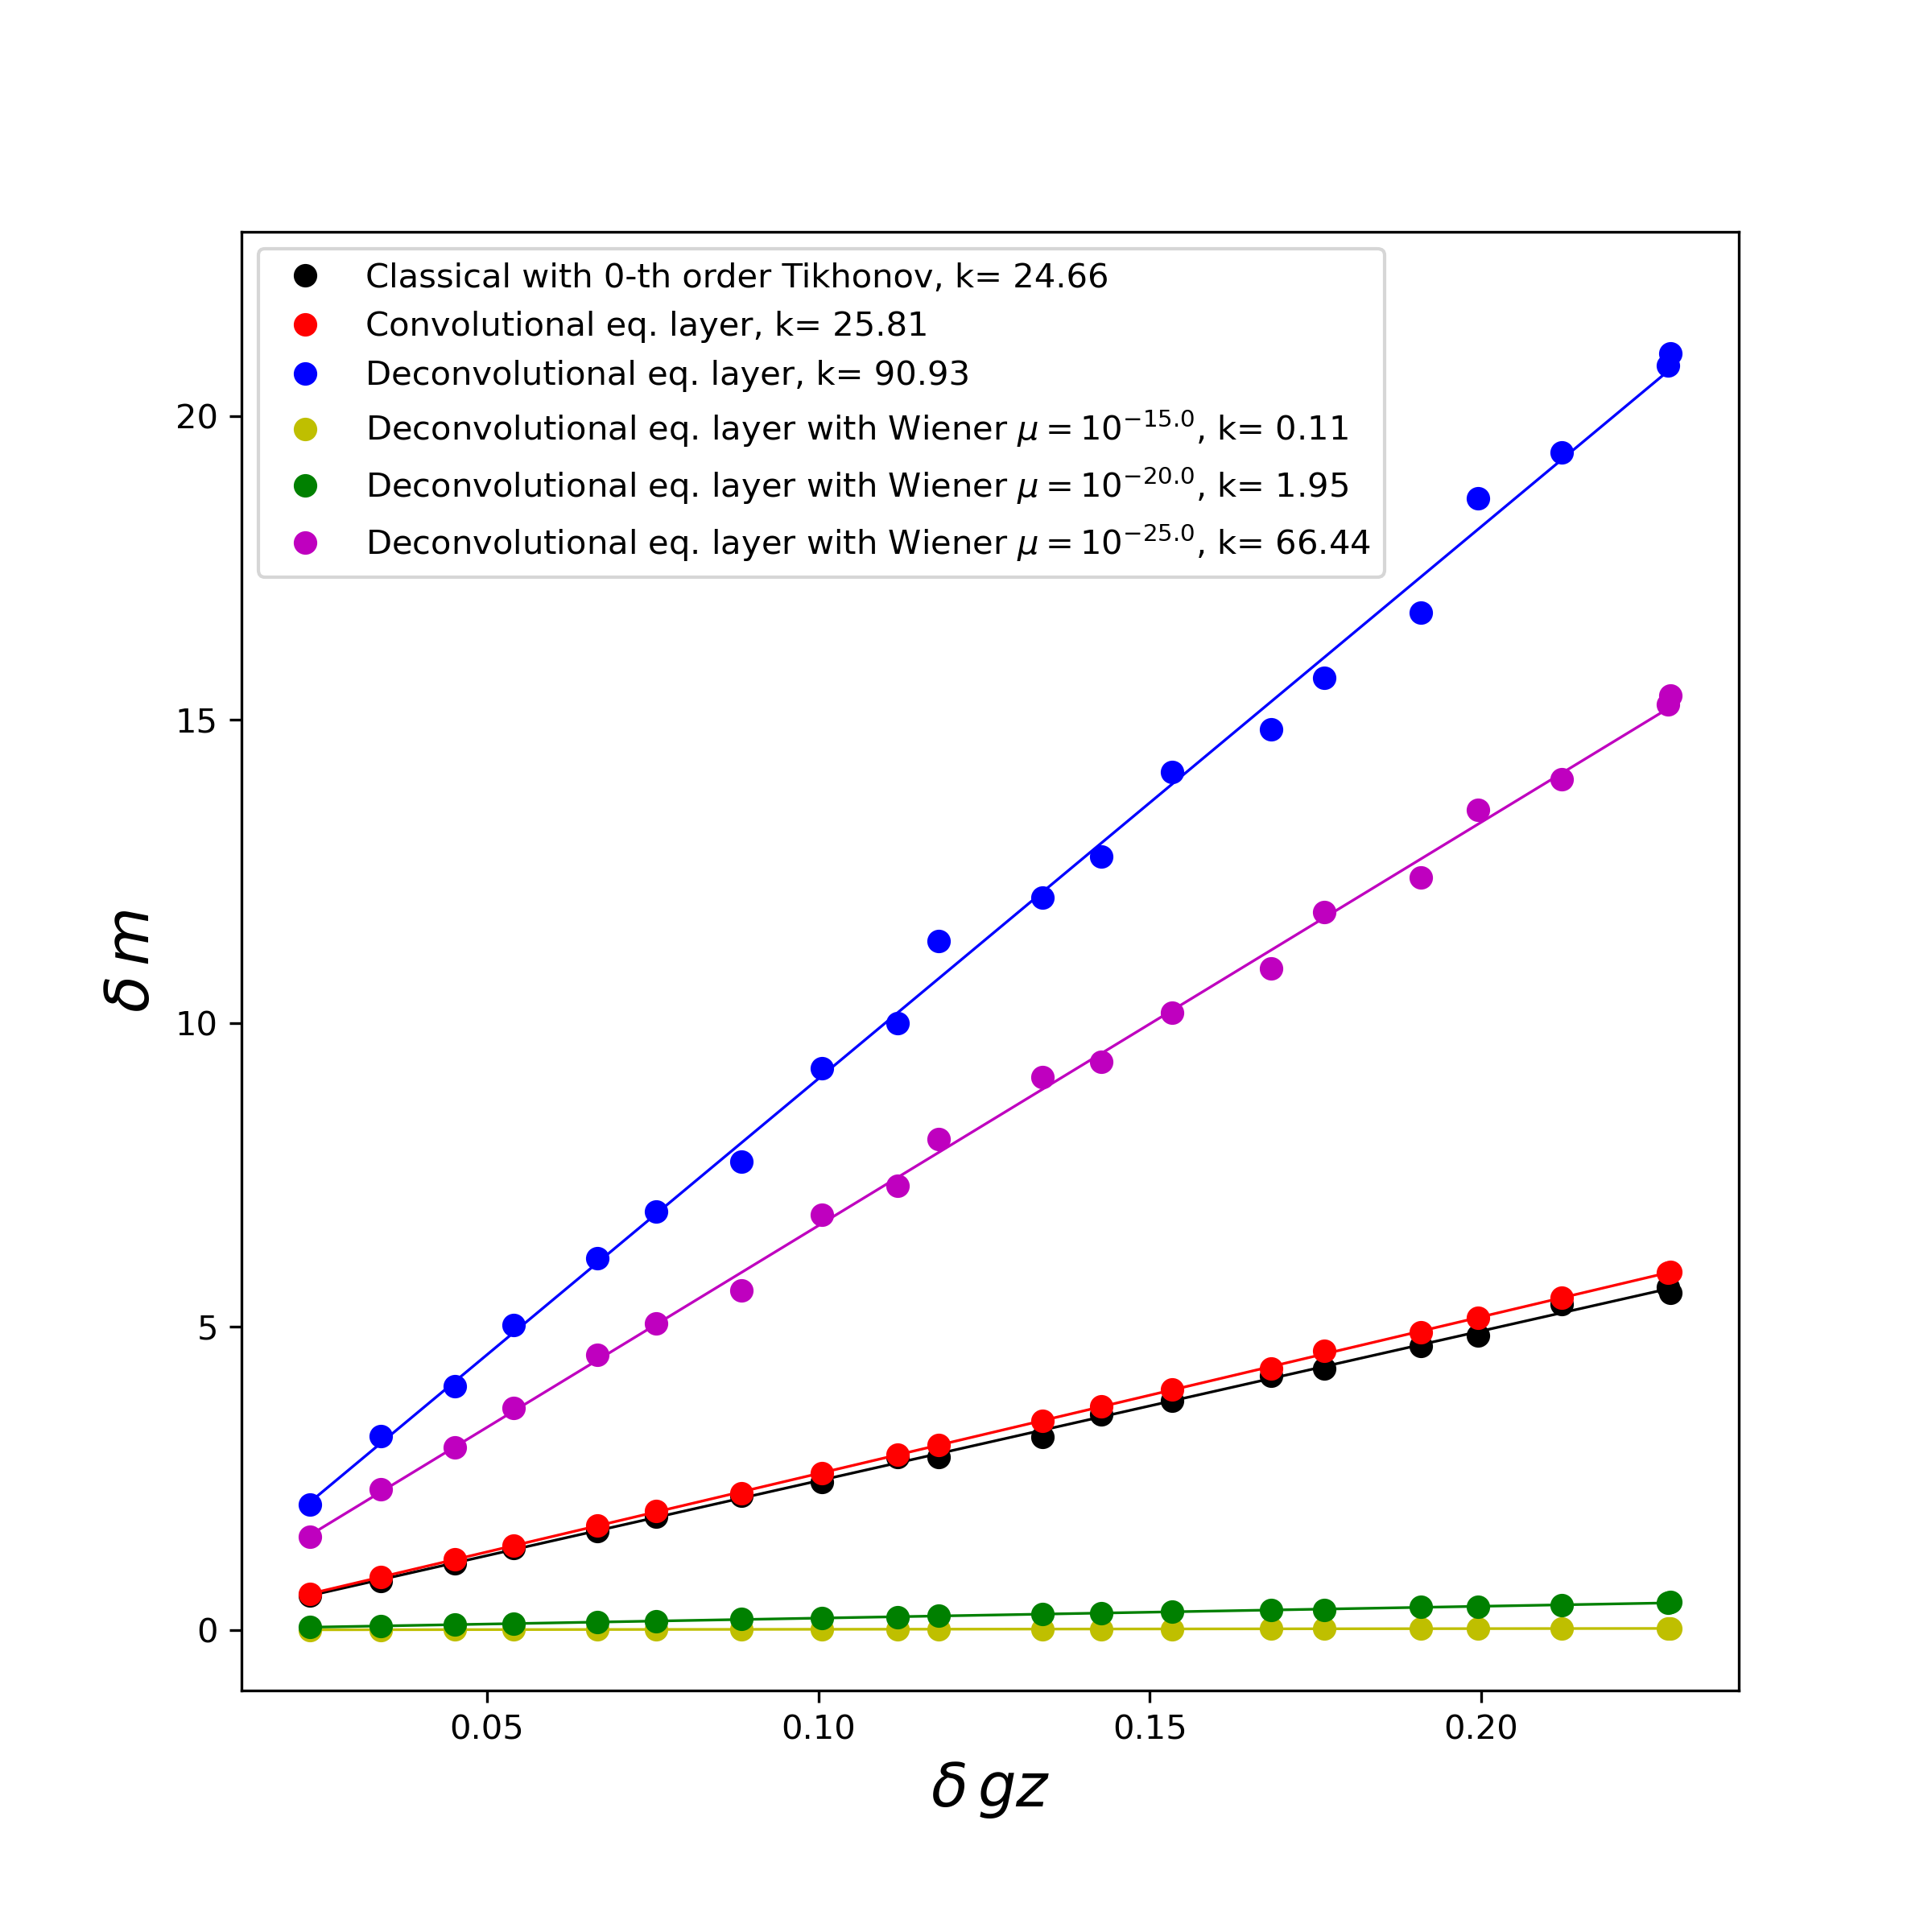
\includegraphics[width=9cm]{Fig/stability_grav}
	\end{center}
	\caption{
		Numerical stability curves obtained for the $21$ synthetic gravity data sets 
		by using the Cholesky factorization with $\mu \approx 10^{-22}$, the iterative deconvolution
		($\mathtt{TOB20}$) proposed by \citet{takahashi-etal2020} with $40$ iterations (Algorithm \ref{alg:TOB20-22}) 
		and the direct deconvolution ($\mathtt{deconv.}$) computed with four different values for $\zeta$ 
		(equation \ref{eq:matrix-L-Wiener-deconvolution}): $0$, $10^{-20}$ (overshoot), $10^{-22}$ (optimal)
		and $10^{-24}$ (suboptimal).
		The stability parameter $\kappa$ (equation \ref{eq:condition-number}) obtained for the six curves
		described above are $24.66$ ($\mathtt{Cholesky}$), $25.81$ ($\mathtt{TOB20}$), $90.93$, $1.95$, $17.47$ and $41.24$ ($\mathtt{deconv.}$ with null, overshoot, optimal and suboptimal $\zeta$).
		}
	\label{fig:3}
\end{figure}

\begin{figure}[htbp]
	\begin{center}
			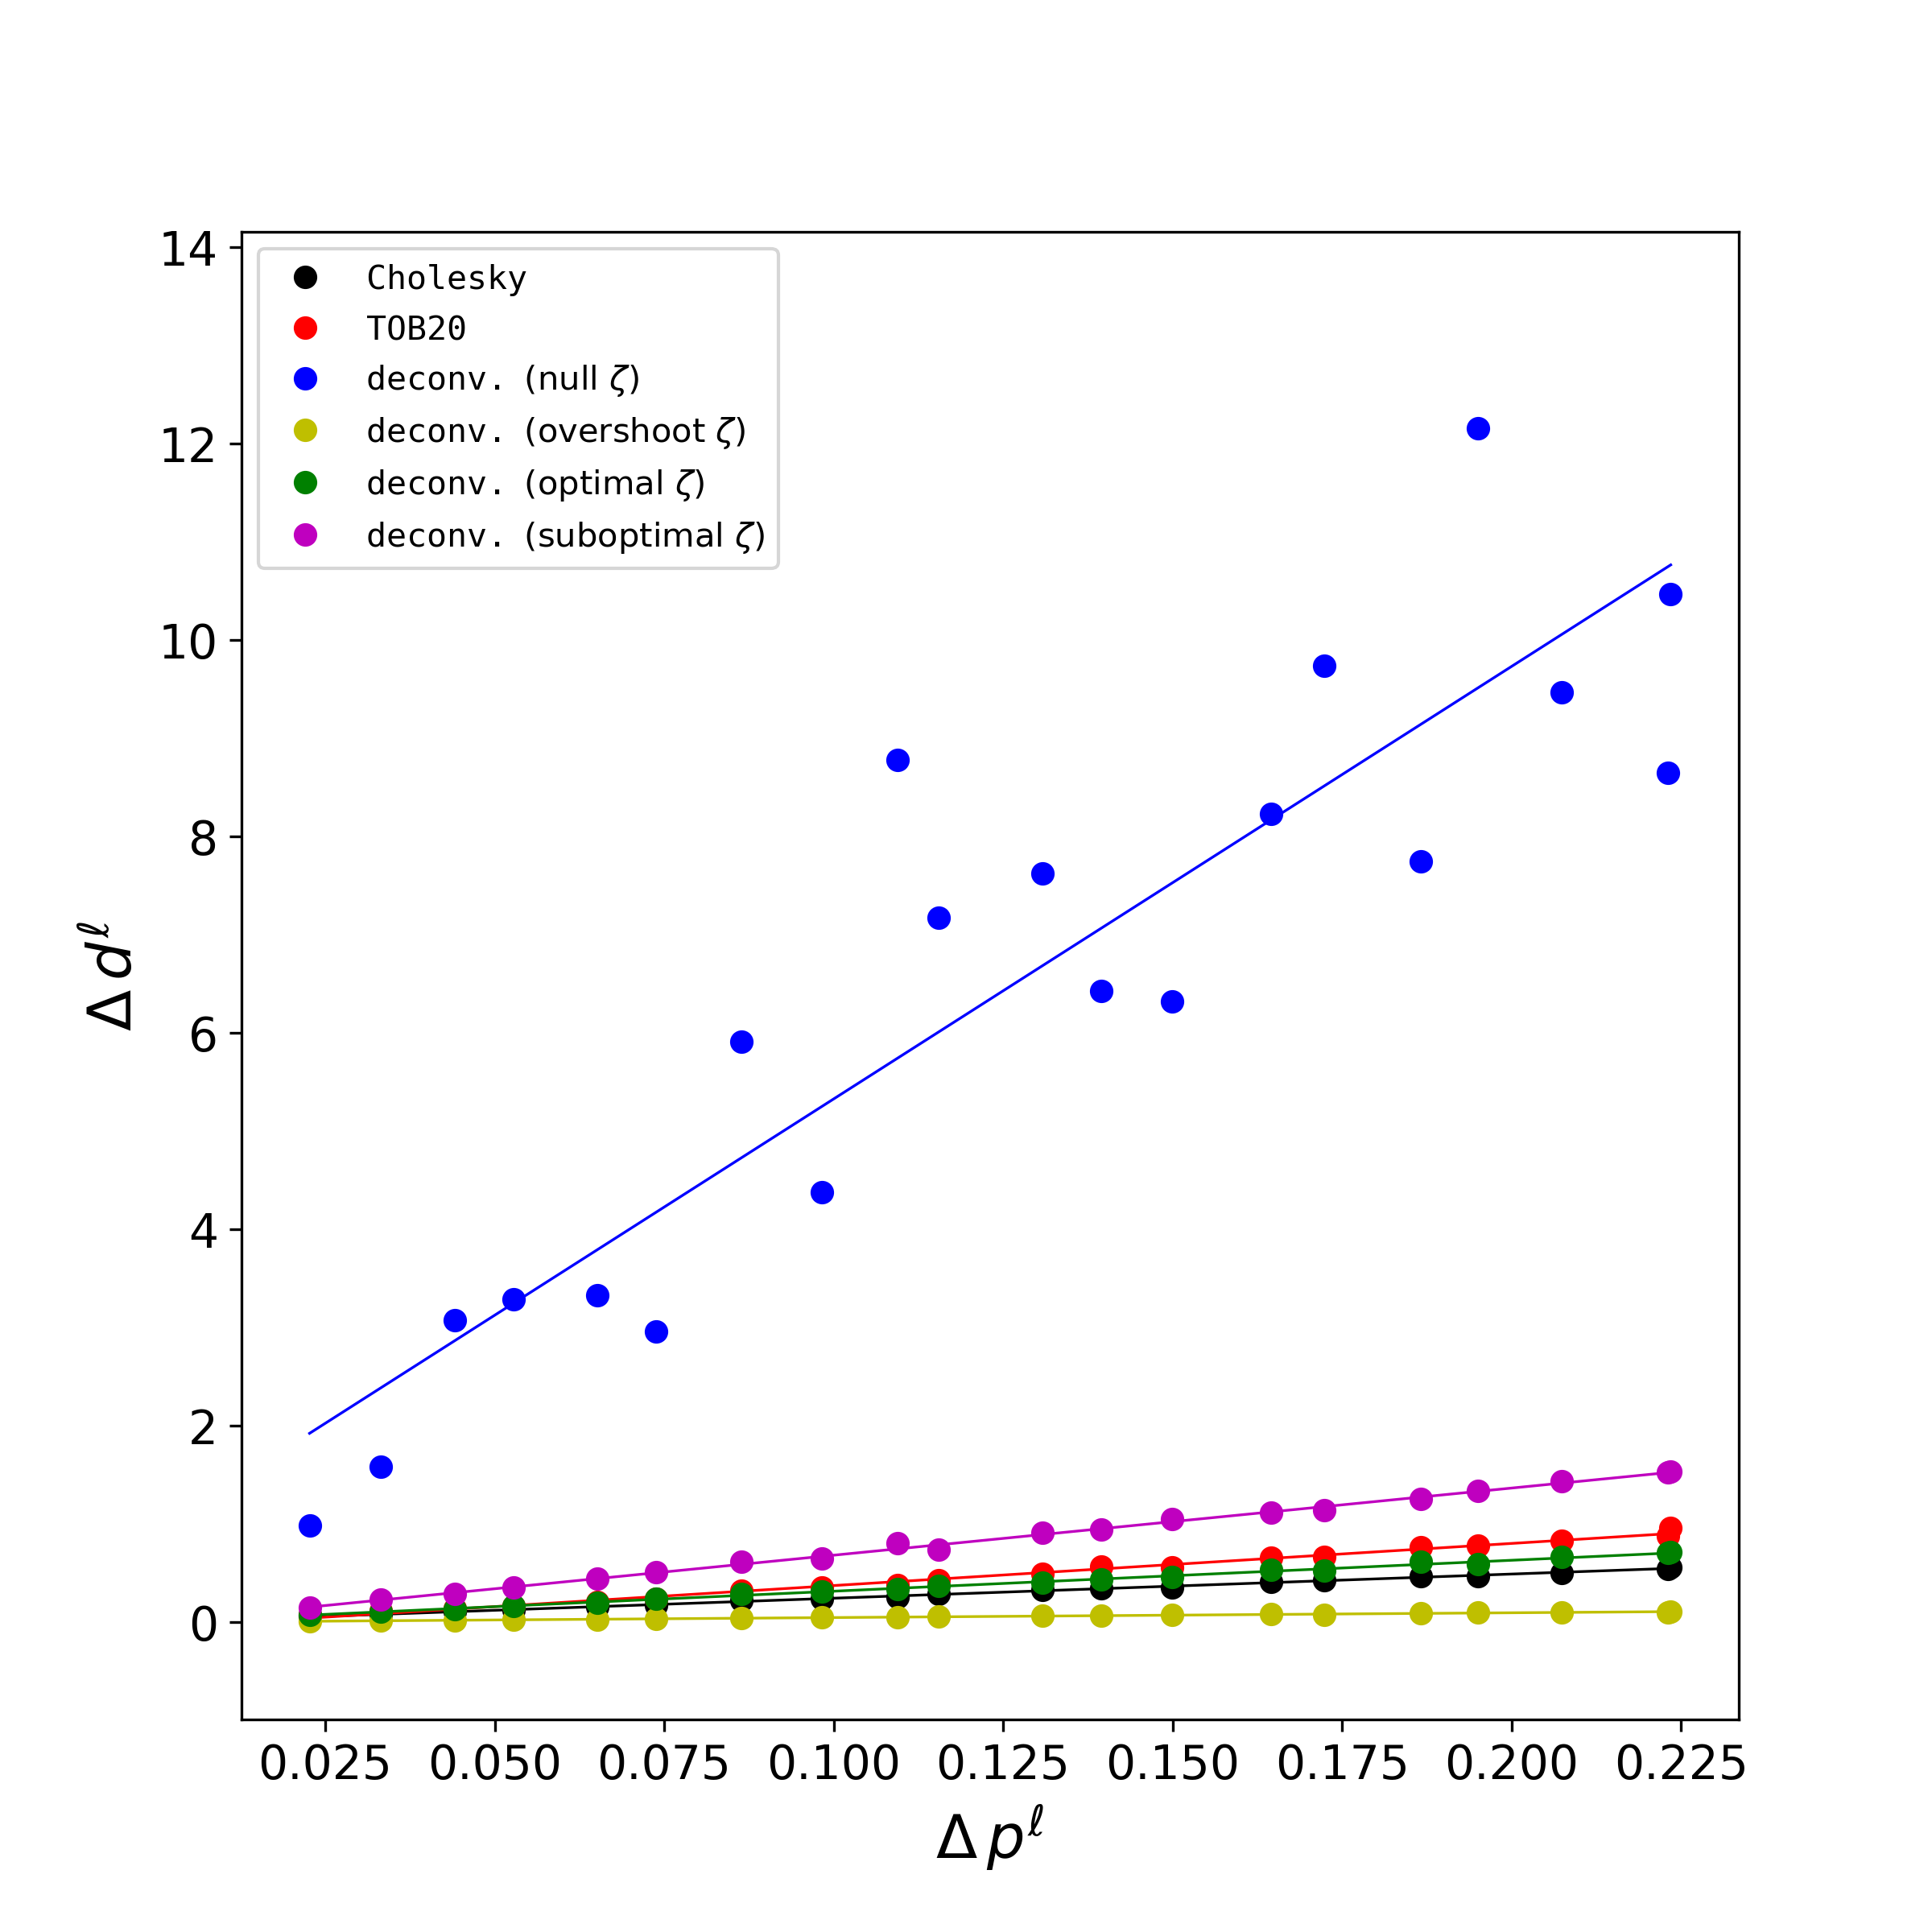
\includegraphics[width=10cm]{Fig/stability_mag}
		\end{center}
	\caption{
		Numerical stability curves obtained for the $21$ synthetic magnetic data sets 
		by using the Cholesky factorization with $\mu \approx 10^{-14}$, the iterative deconvolution
		($\mathtt{TOB20}$) proposed by \citet{takahashi-etal2022} with $40$ iterations (Algorithm \ref{alg:TOB20-22}) 
		and the direct deconvolution ($\mathtt{deconv.}$) computed with four different values for $\zeta$ 
		(equation \ref{eq:matrix-L-Wiener-deconvolution}): $0$, $10^{-12}$ (overshoot), $10^{-14}$ (optimal)
		and $10^{-16}$ (suboptimal).
		The stability parameter $\kappa$ (equation \ref{eq:condition-number}) obtained for the six curves
		described above are $2.46$ ($\mathtt{Cholesky}$), $4.29$ ($\mathtt{TOB20}$), $44.04$, $0.49$, $3.15$ and $6.83$ ($\mathtt{deconv.}$ with null, overshoot, optimal and suboptimal $\zeta$).
		}
	\label{fig:6}
\end{figure}

\begin{figure}[htbp]
	\begin{center}
		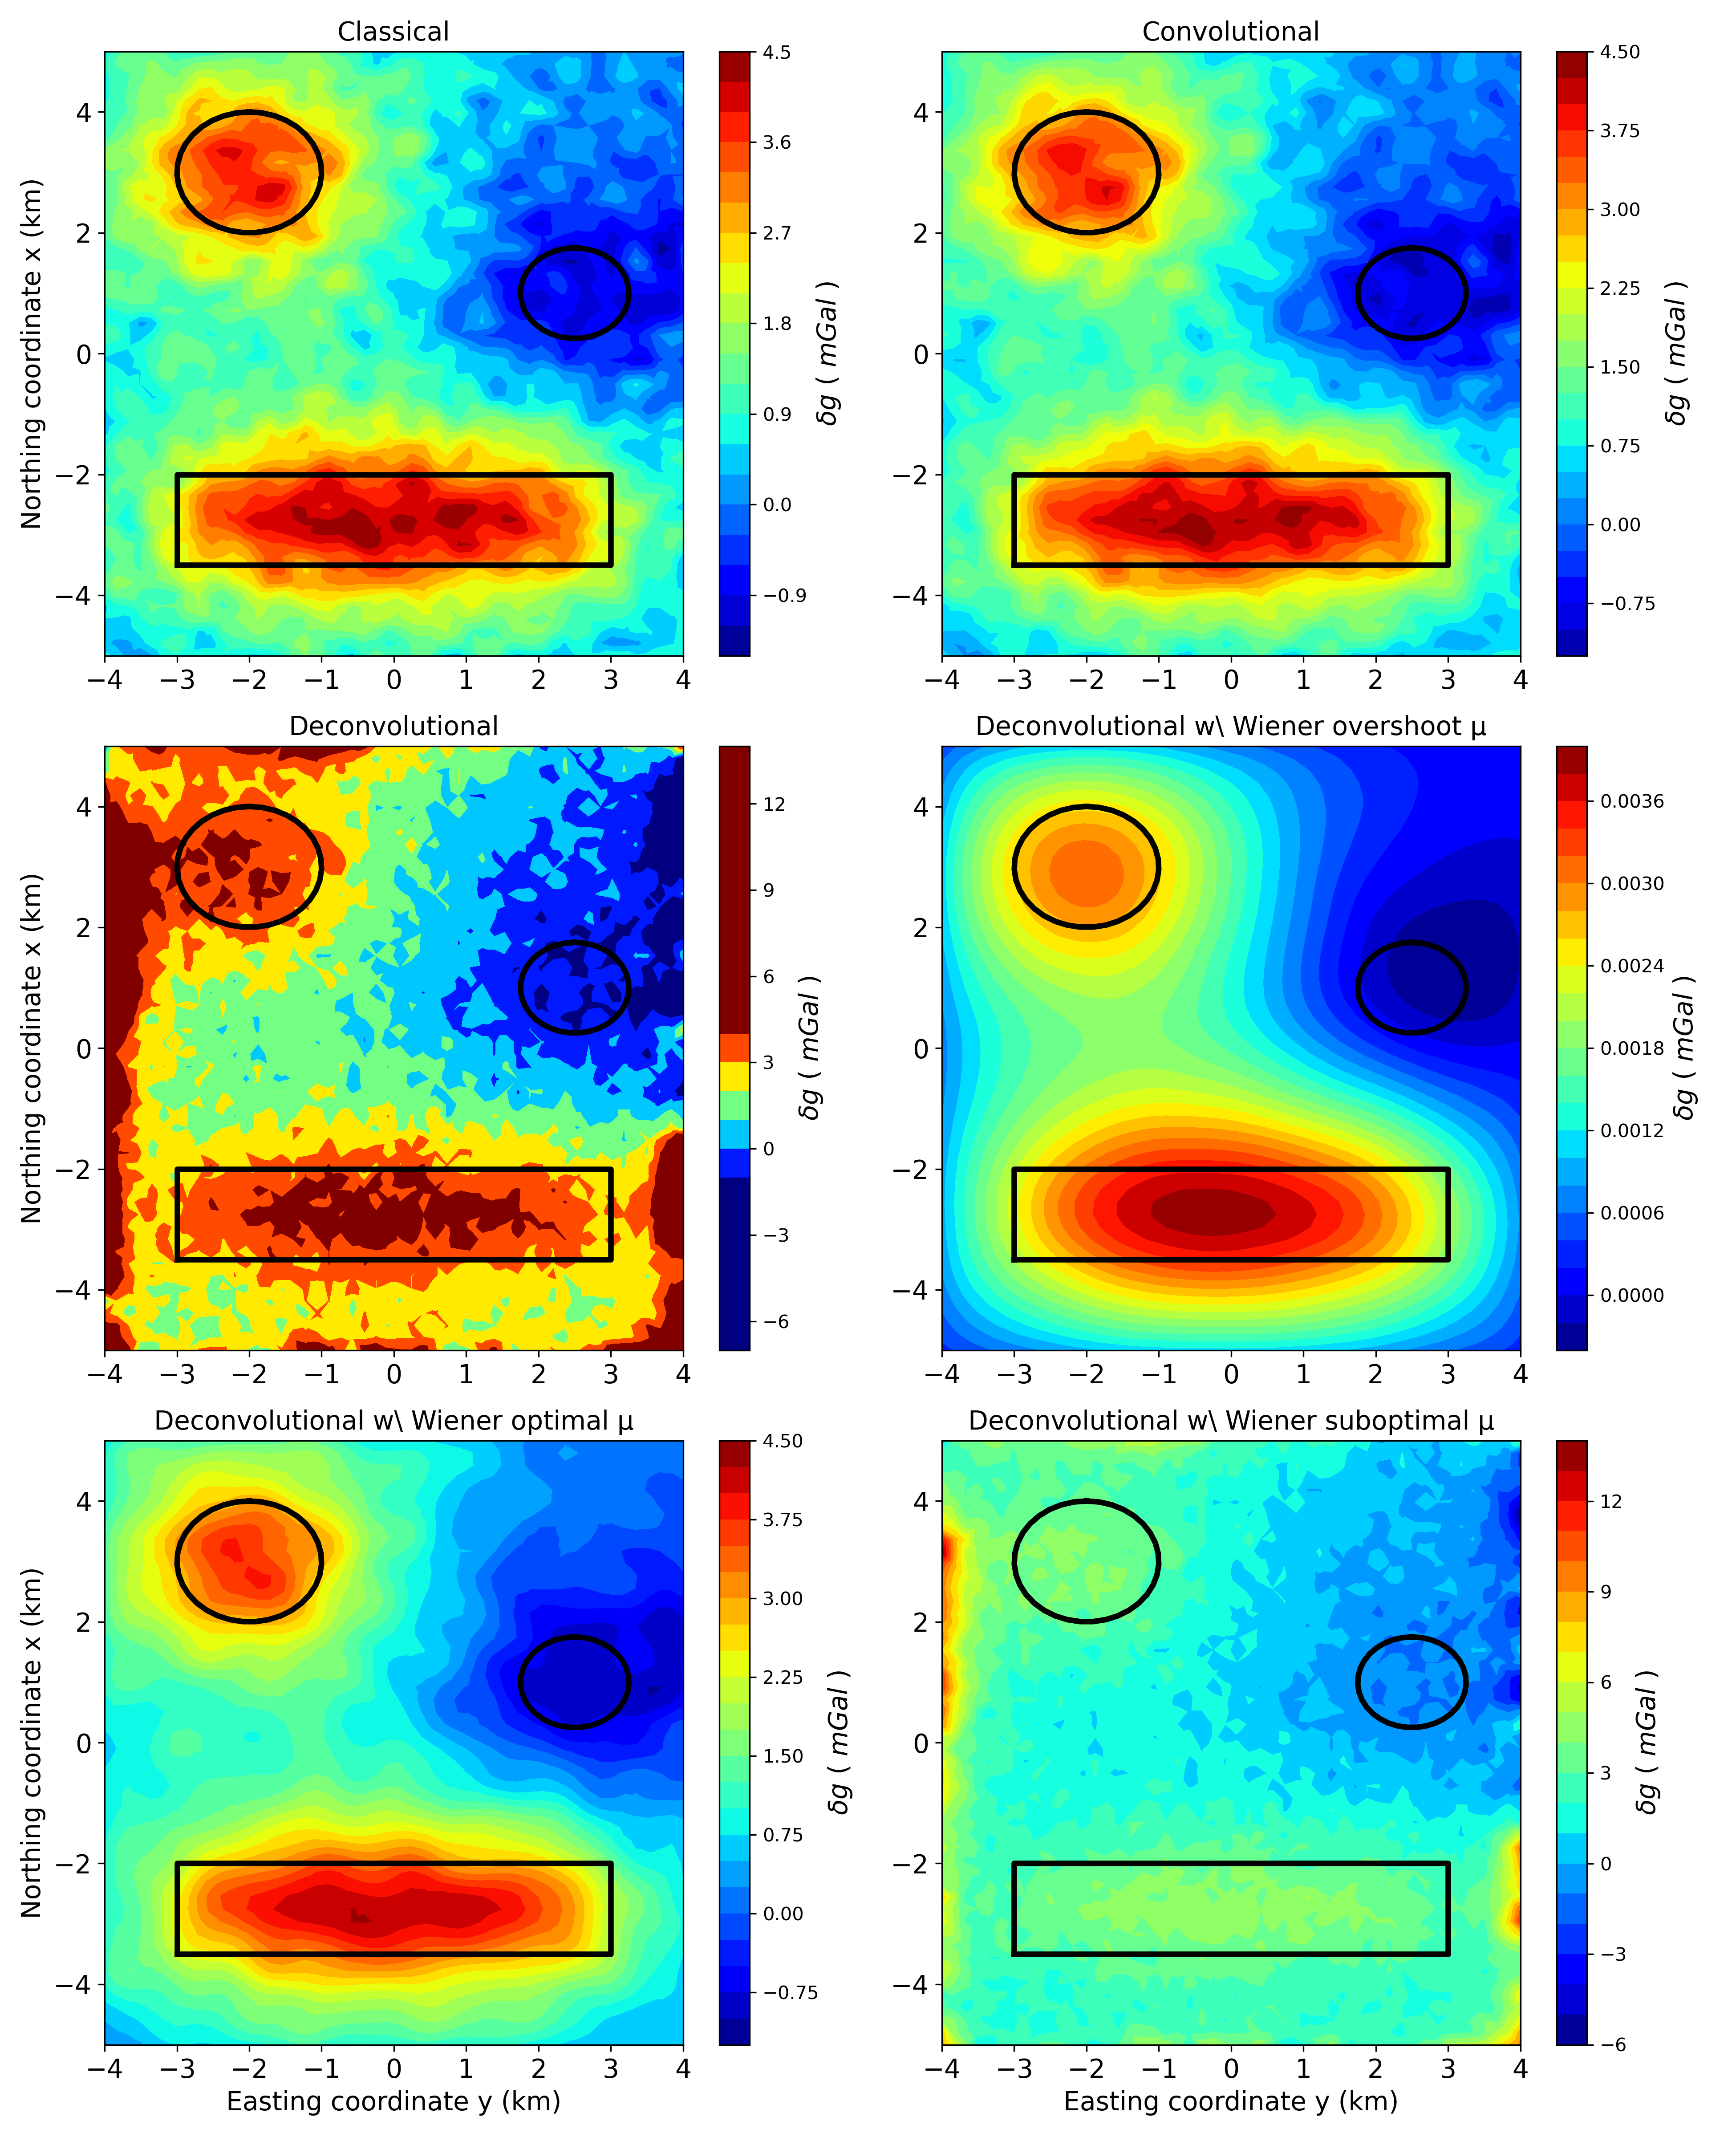
\includegraphics[width=10cm]{Fig/stability_grav_comparison}
	\end{center}
	\caption{
		Predicted data $\mathbf{f}$ (equation \ref{eq:predicted-data-vector}) due to the estimated parameter vector
		$\tilde{\mathbf{p}}$ obtained with the gravity data having maximum noise level (Figure \ref{fig:4}B) by using
		\textbf{(A)} the Cholesky factorization with $\mu \approx 10^{-22}$, 
		\textbf{(B)} the iterative deconvolution ($\mathtt{TOB20}$) proposed by \citet{takahashi-etal2020} with $40$ 
		iterations (Algorithm \ref{alg:TOB20-22}) and
		\textbf{(C)}--\textbf{(F)} the direct deconvolution ($\mathtt{deconv.}$) computed, respectively, with four different 
		values for $\zeta$ (equation \ref{eq:matrix-L-Wiener-deconvolution}): $0$, $10^{-20}$ (overshoot), $10^{-22}$ (optimal)
		and $10^{-24}$ (suboptimal).
		All values are in $\mathrm{mGal}$.
		}
	\label{fig:5}
\end{figure}

\begin{figure}[htbp]
	\begin{center}
		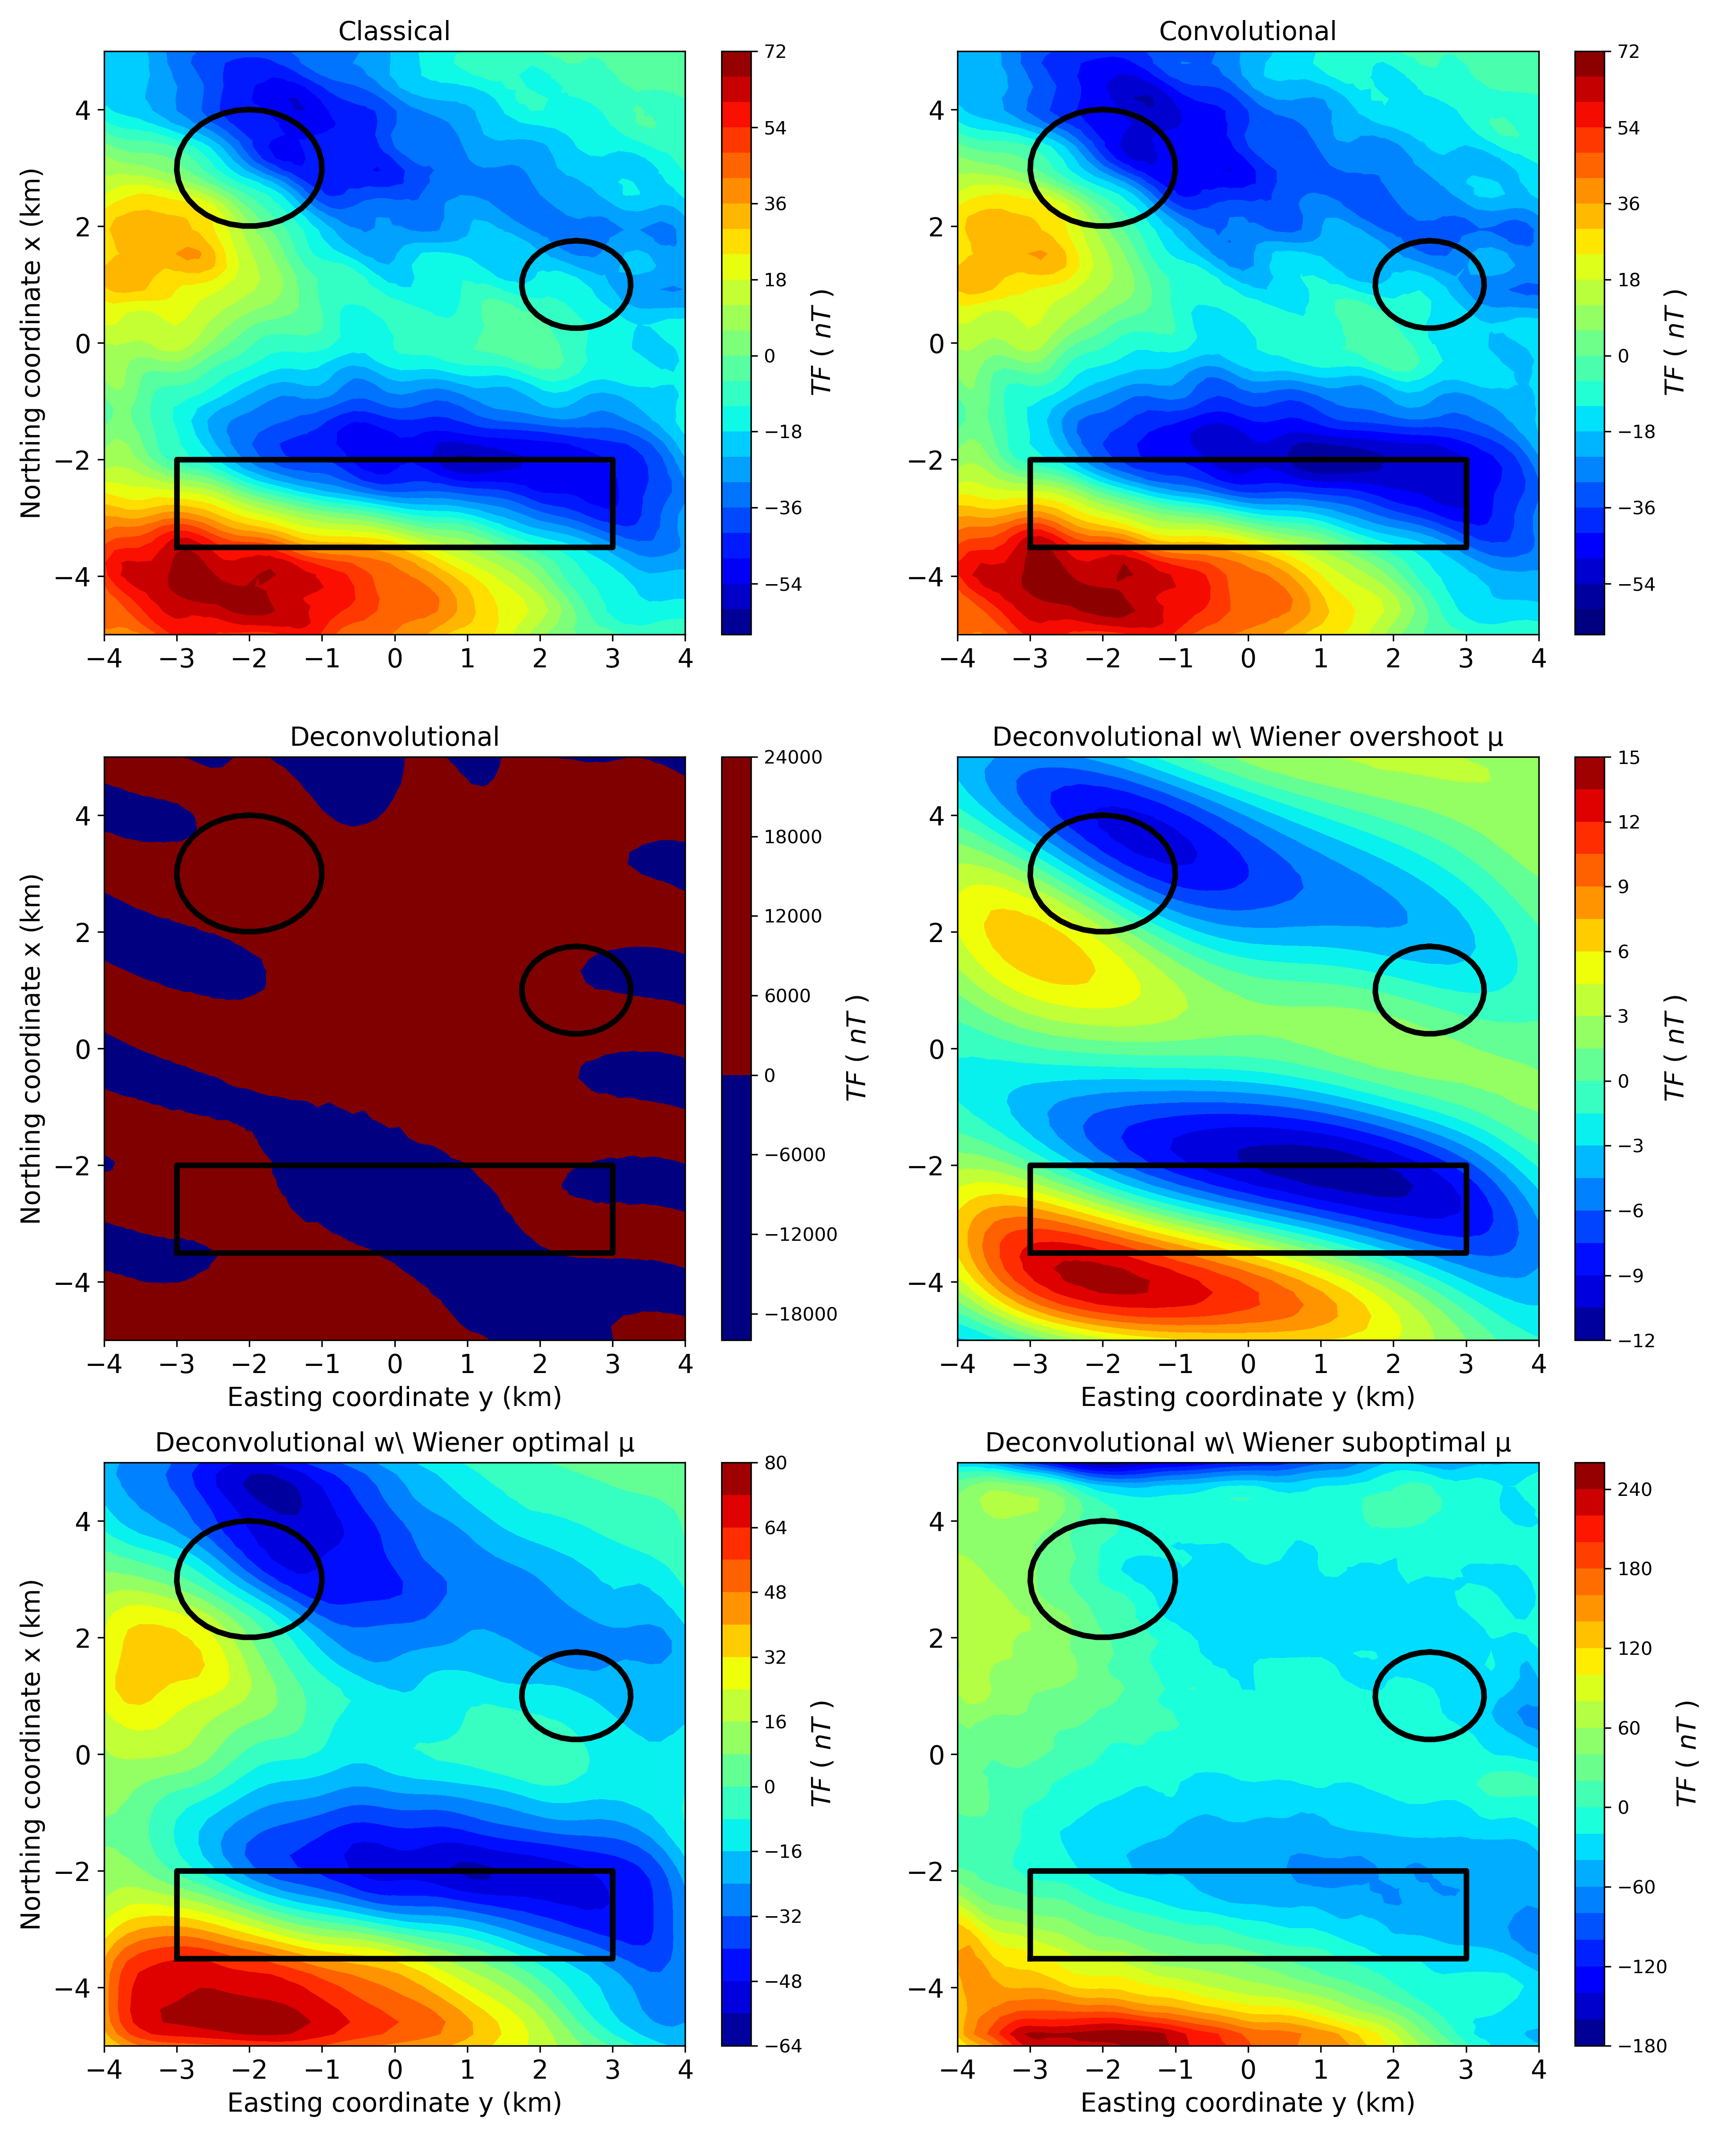
\includegraphics[width=10cm]{Fig/stability_mag_comparison}
	\end{center}
	\caption{
		Predicted data $\mathbf{f}$ (equation \ref{eq:predicted-data-vector}) due to the estimated parameter vector
		$\tilde{\mathbf{p}}$ obtained with the magnetic data having maximum noise level (Figure \ref{fig:7}B) by using
		\textbf{(A)} the Cholesky factorization with $\mu \approx 10^{-14}$, 
		\textbf{(B)} the iterative deconvolution ($\mathtt{TOB20}$) proposed by \citet{takahashi-etal2022} with $40$ 
		iterations (Algorithm \ref{alg:TOB20-22}) and
		\textbf{(C)}--\textbf{(F)} the direct deconvolution ($\mathtt{deconv.}$) computed with four different 
		values for $\zeta$ (equation \ref{eq:matrix-L-Wiener-deconvolution}): $0$, $10^{-12}$ (overshoot), $10^{-14}$ (optimal)
		and $10^{-16}$ (suboptimal).
		All values are in $\mathrm{nT}$.
		}
	\label{fig:8}
\end{figure}

\begin{figure}[htbp]
	\begin{center}
		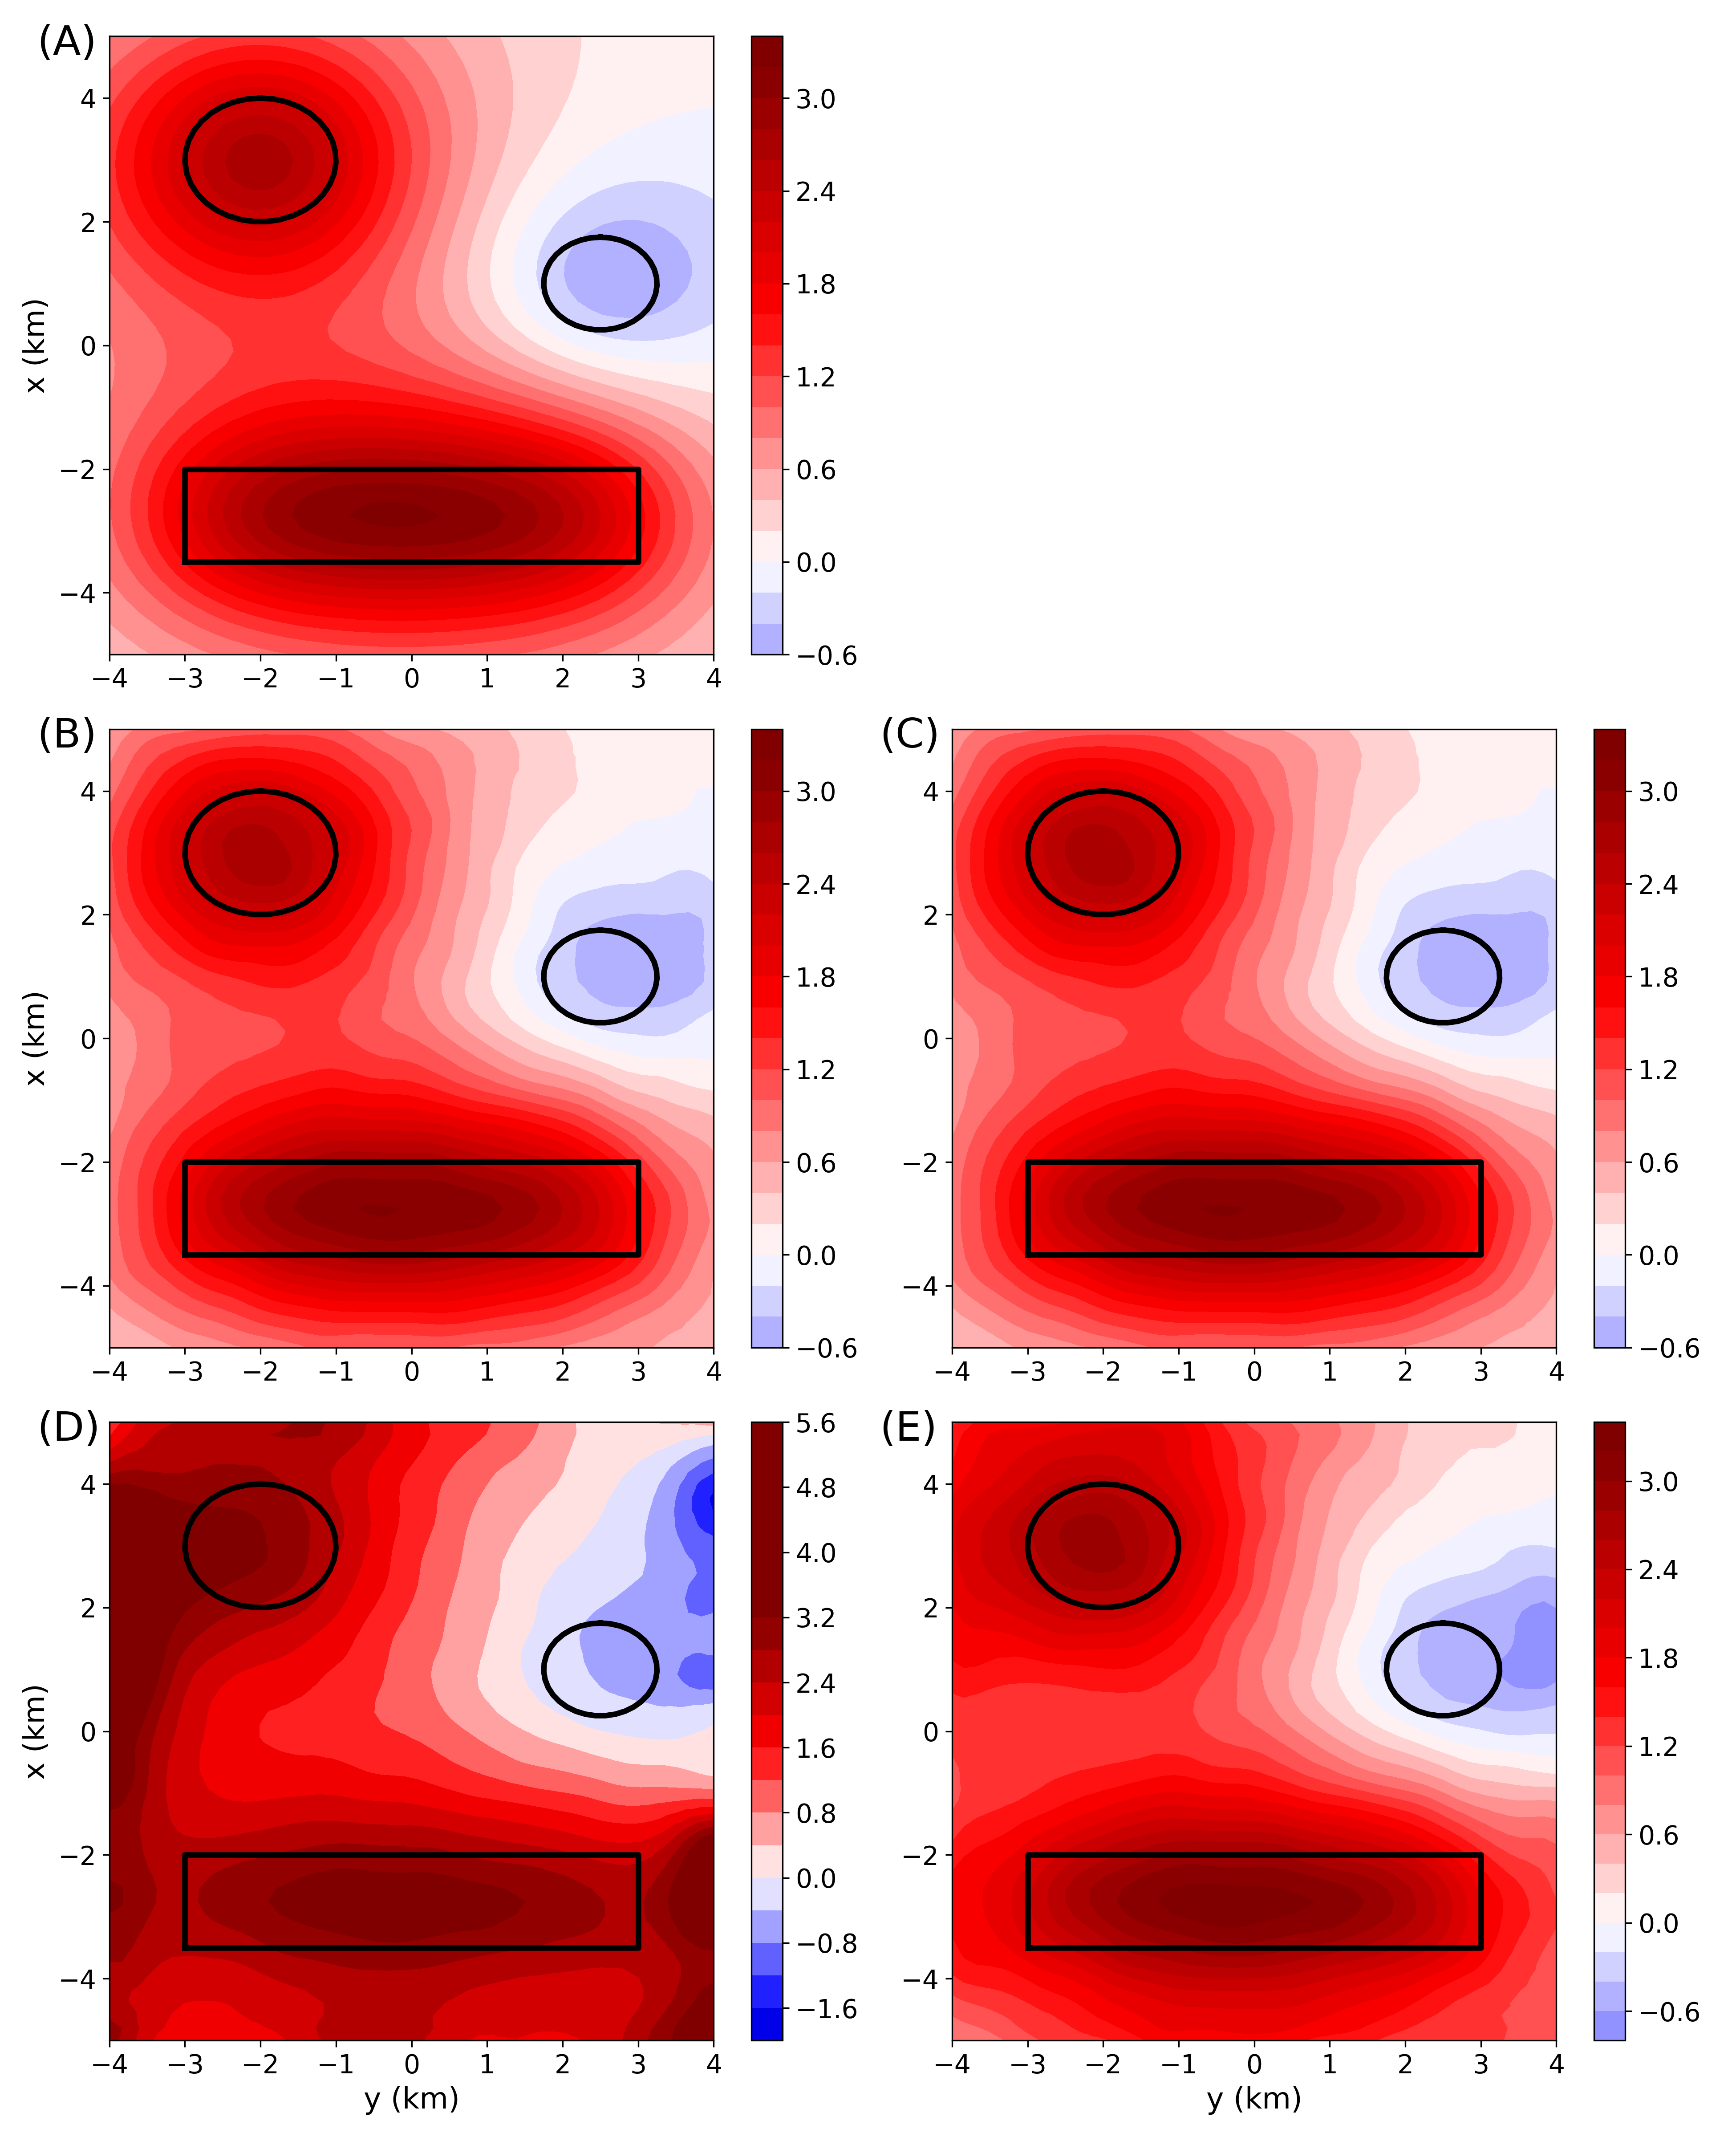
\includegraphics[width=10cm]{Fig/grav_upward}
	\end{center}
	\caption{
		Upward continuation of the synthetic gravity data with maximum noise level (Figure \ref{fig:4}B).
		\textbf{(A)} Noise-free gravity data produced by the model at $z = -500 \: \mathrm{m}$. 
		\textbf{(B)}--\textbf{(E)} Continued data due to the estimated parameter vector $\tilde{\mathbf{p}}$ obtained, respectively,
		by using the Cholesky factorization with $\mu \approx 10^{-22}$, 
		the iterative deconvolution ($\mathtt{TOB20}$) proposed by \citet{takahashi-etal2020} with $40$ 
		iterations (Algorithm \ref{alg:TOB20-22}) and
		the direct deconvolution ($\mathtt{deconv.}$) computed, respectively, with two different 
		values for $\zeta$ (equation \ref{eq:matrix-L-Wiener-deconvolution}): $0$ and $10^{-22}$ (optimal).
		All values are in $\mathrm{mGal}$.
		}
	\label{fig:grav_up}
\end{figure}

\begin{figure}[htbp]
	\begin{center}
		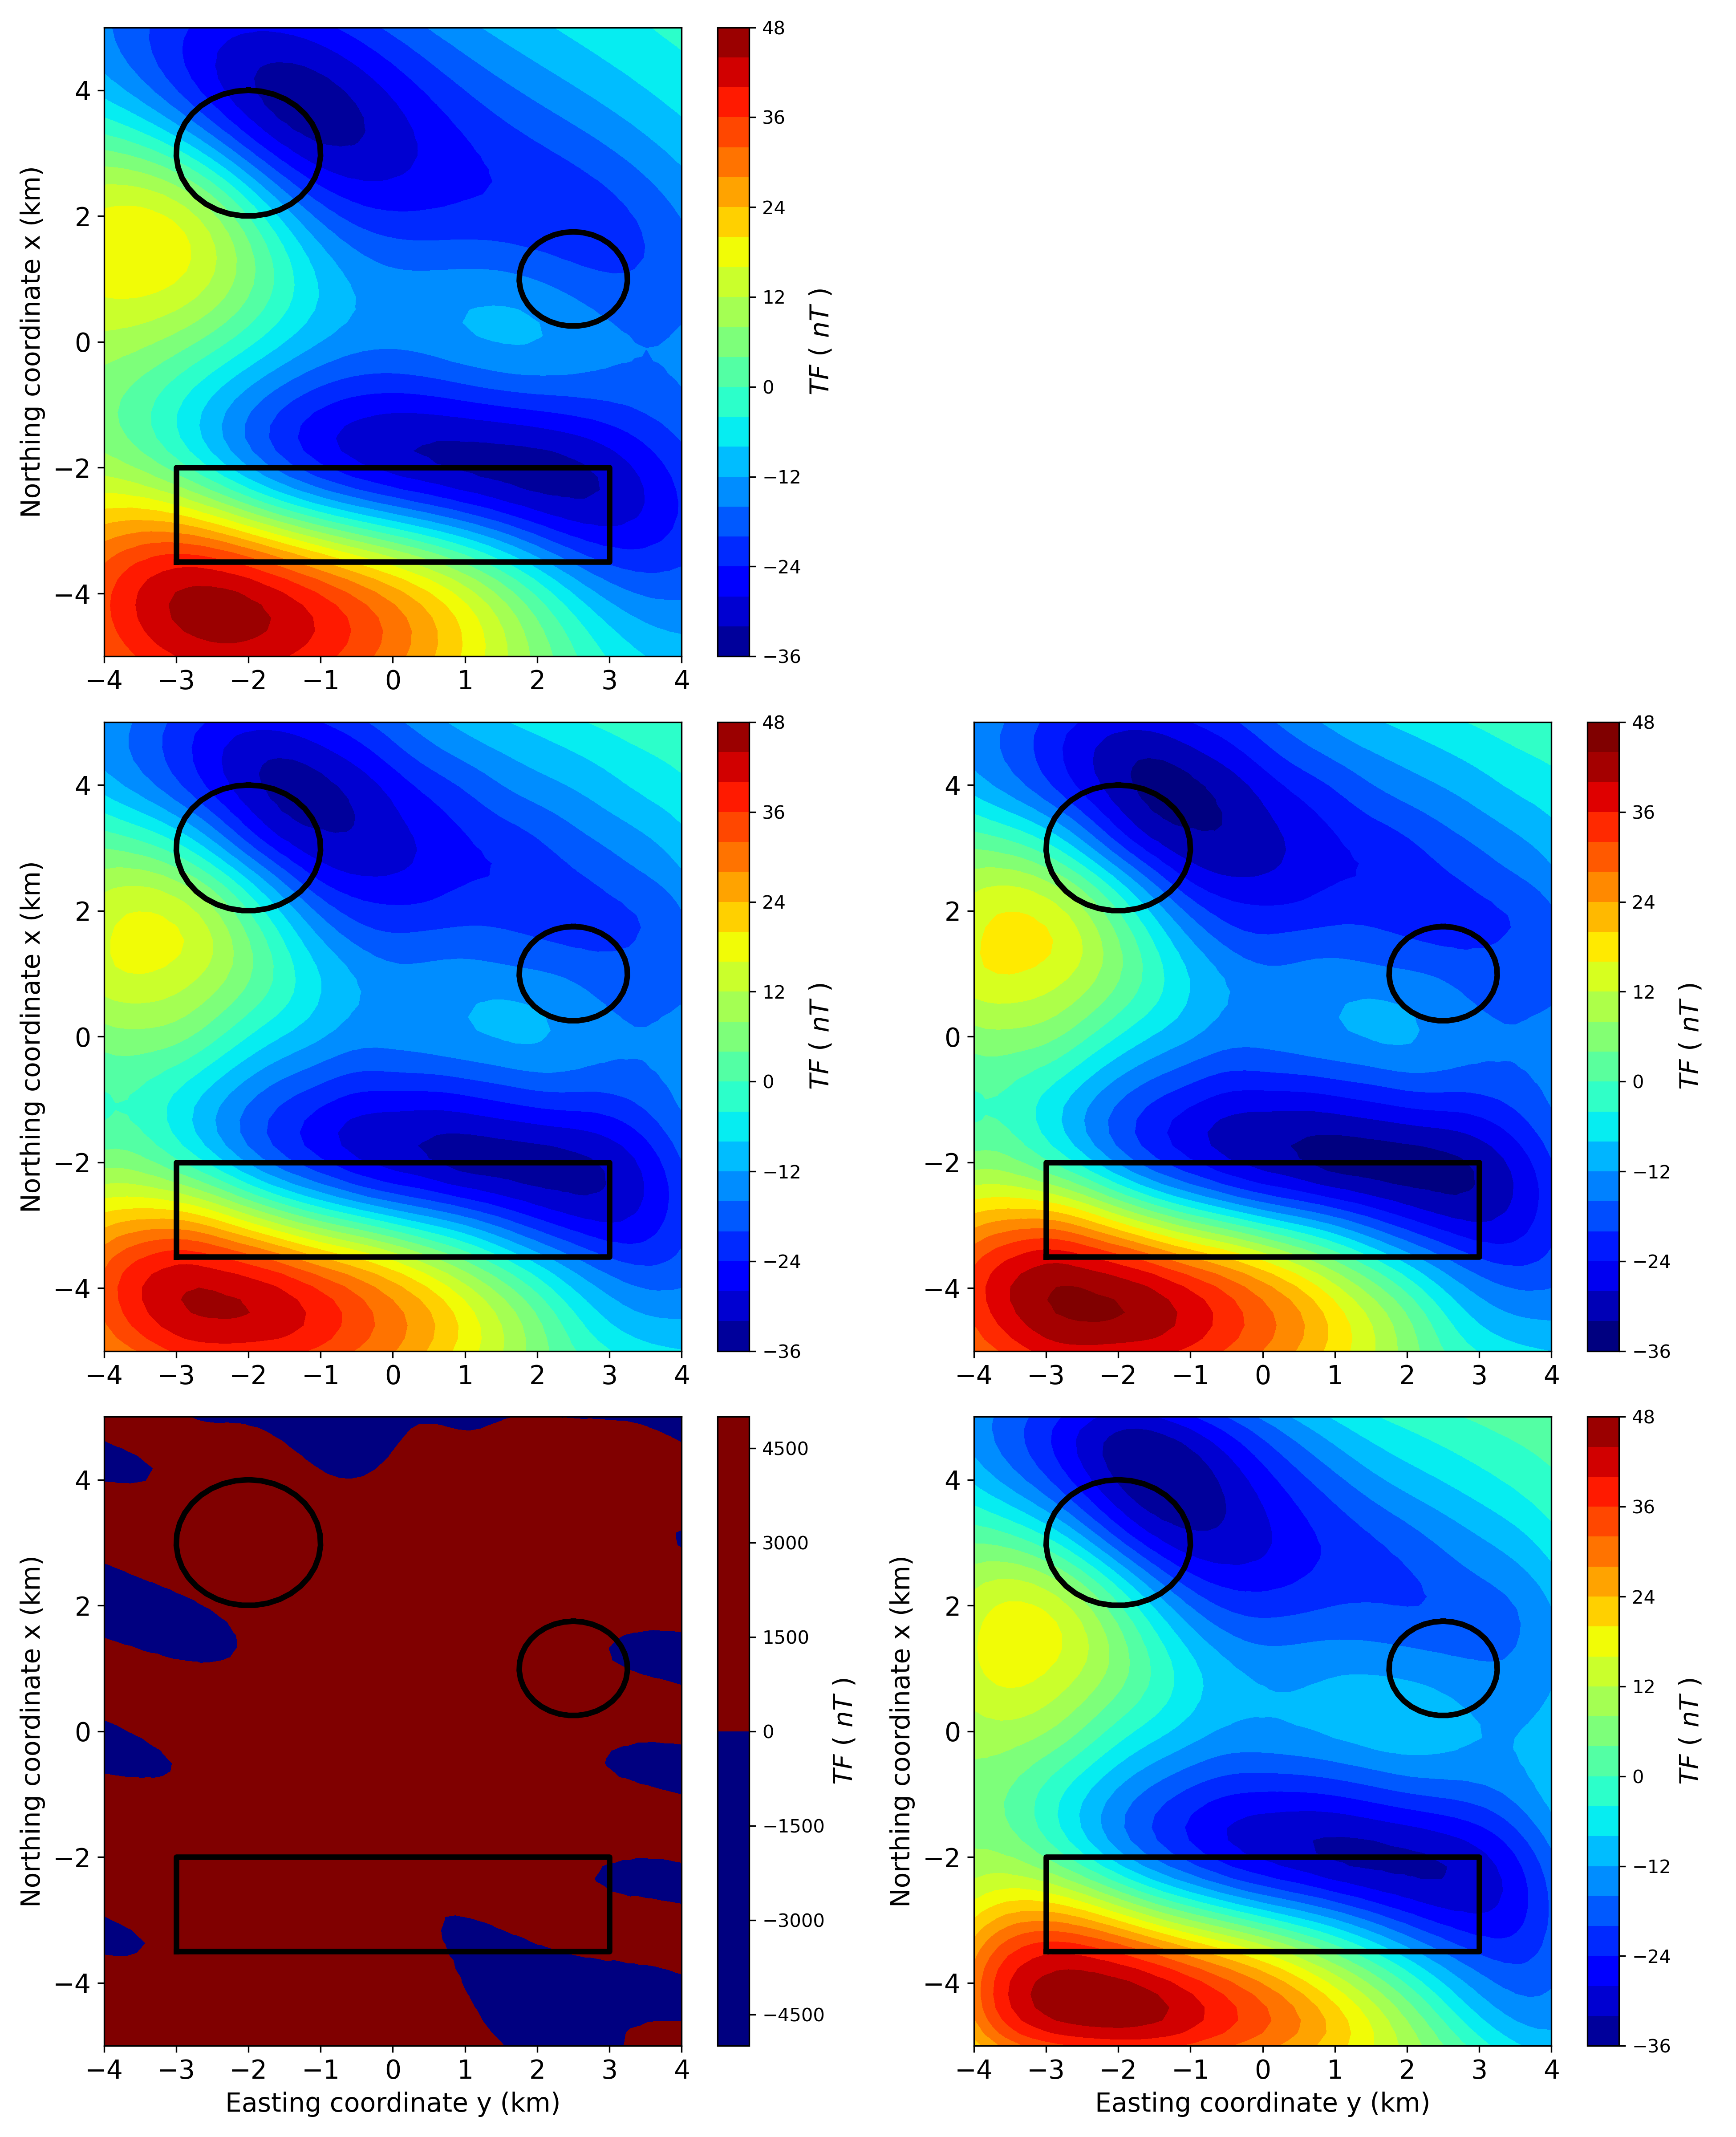
\includegraphics[width=10cm]{Fig/mag_upward}
	\end{center}
	\caption{
		Upward continuation of the synthetic magnetic data with maximum noise level (Figure \ref{fig:7}B).
		\textbf{(A)} Noise-free magnetic data produced by the model at $z = -1400 \: \mathrm{m}$. 
		\textbf{(B)}--\textbf{(E)} Continued data due to the estimated parameter vector $\tilde{\mathbf{p}}$ obtained, respectively,
		by using the Cholesky factorization with $\mu \approx 10^{-14}$, 
		the iterative deconvolution ($\mathtt{TOB20}$) proposed by \citet{takahashi-etal2022} with $40$ 
		iterations (Algorithm \ref{alg:TOB20-22}) and
		the direct deconvolution ($\mathtt{deconv.}$) computed, respectively, with two different 
		values for $\zeta$ (equation \ref{eq:matrix-L-Wiener-deconvolution}): $0$ and $10^{-14}$ (optimal).
		All values are in $\mathrm{nT}$.
		}
	\label{fig:mag_up}
\end{figure}

\begin{figure}[htbp]
	\begin{center}
		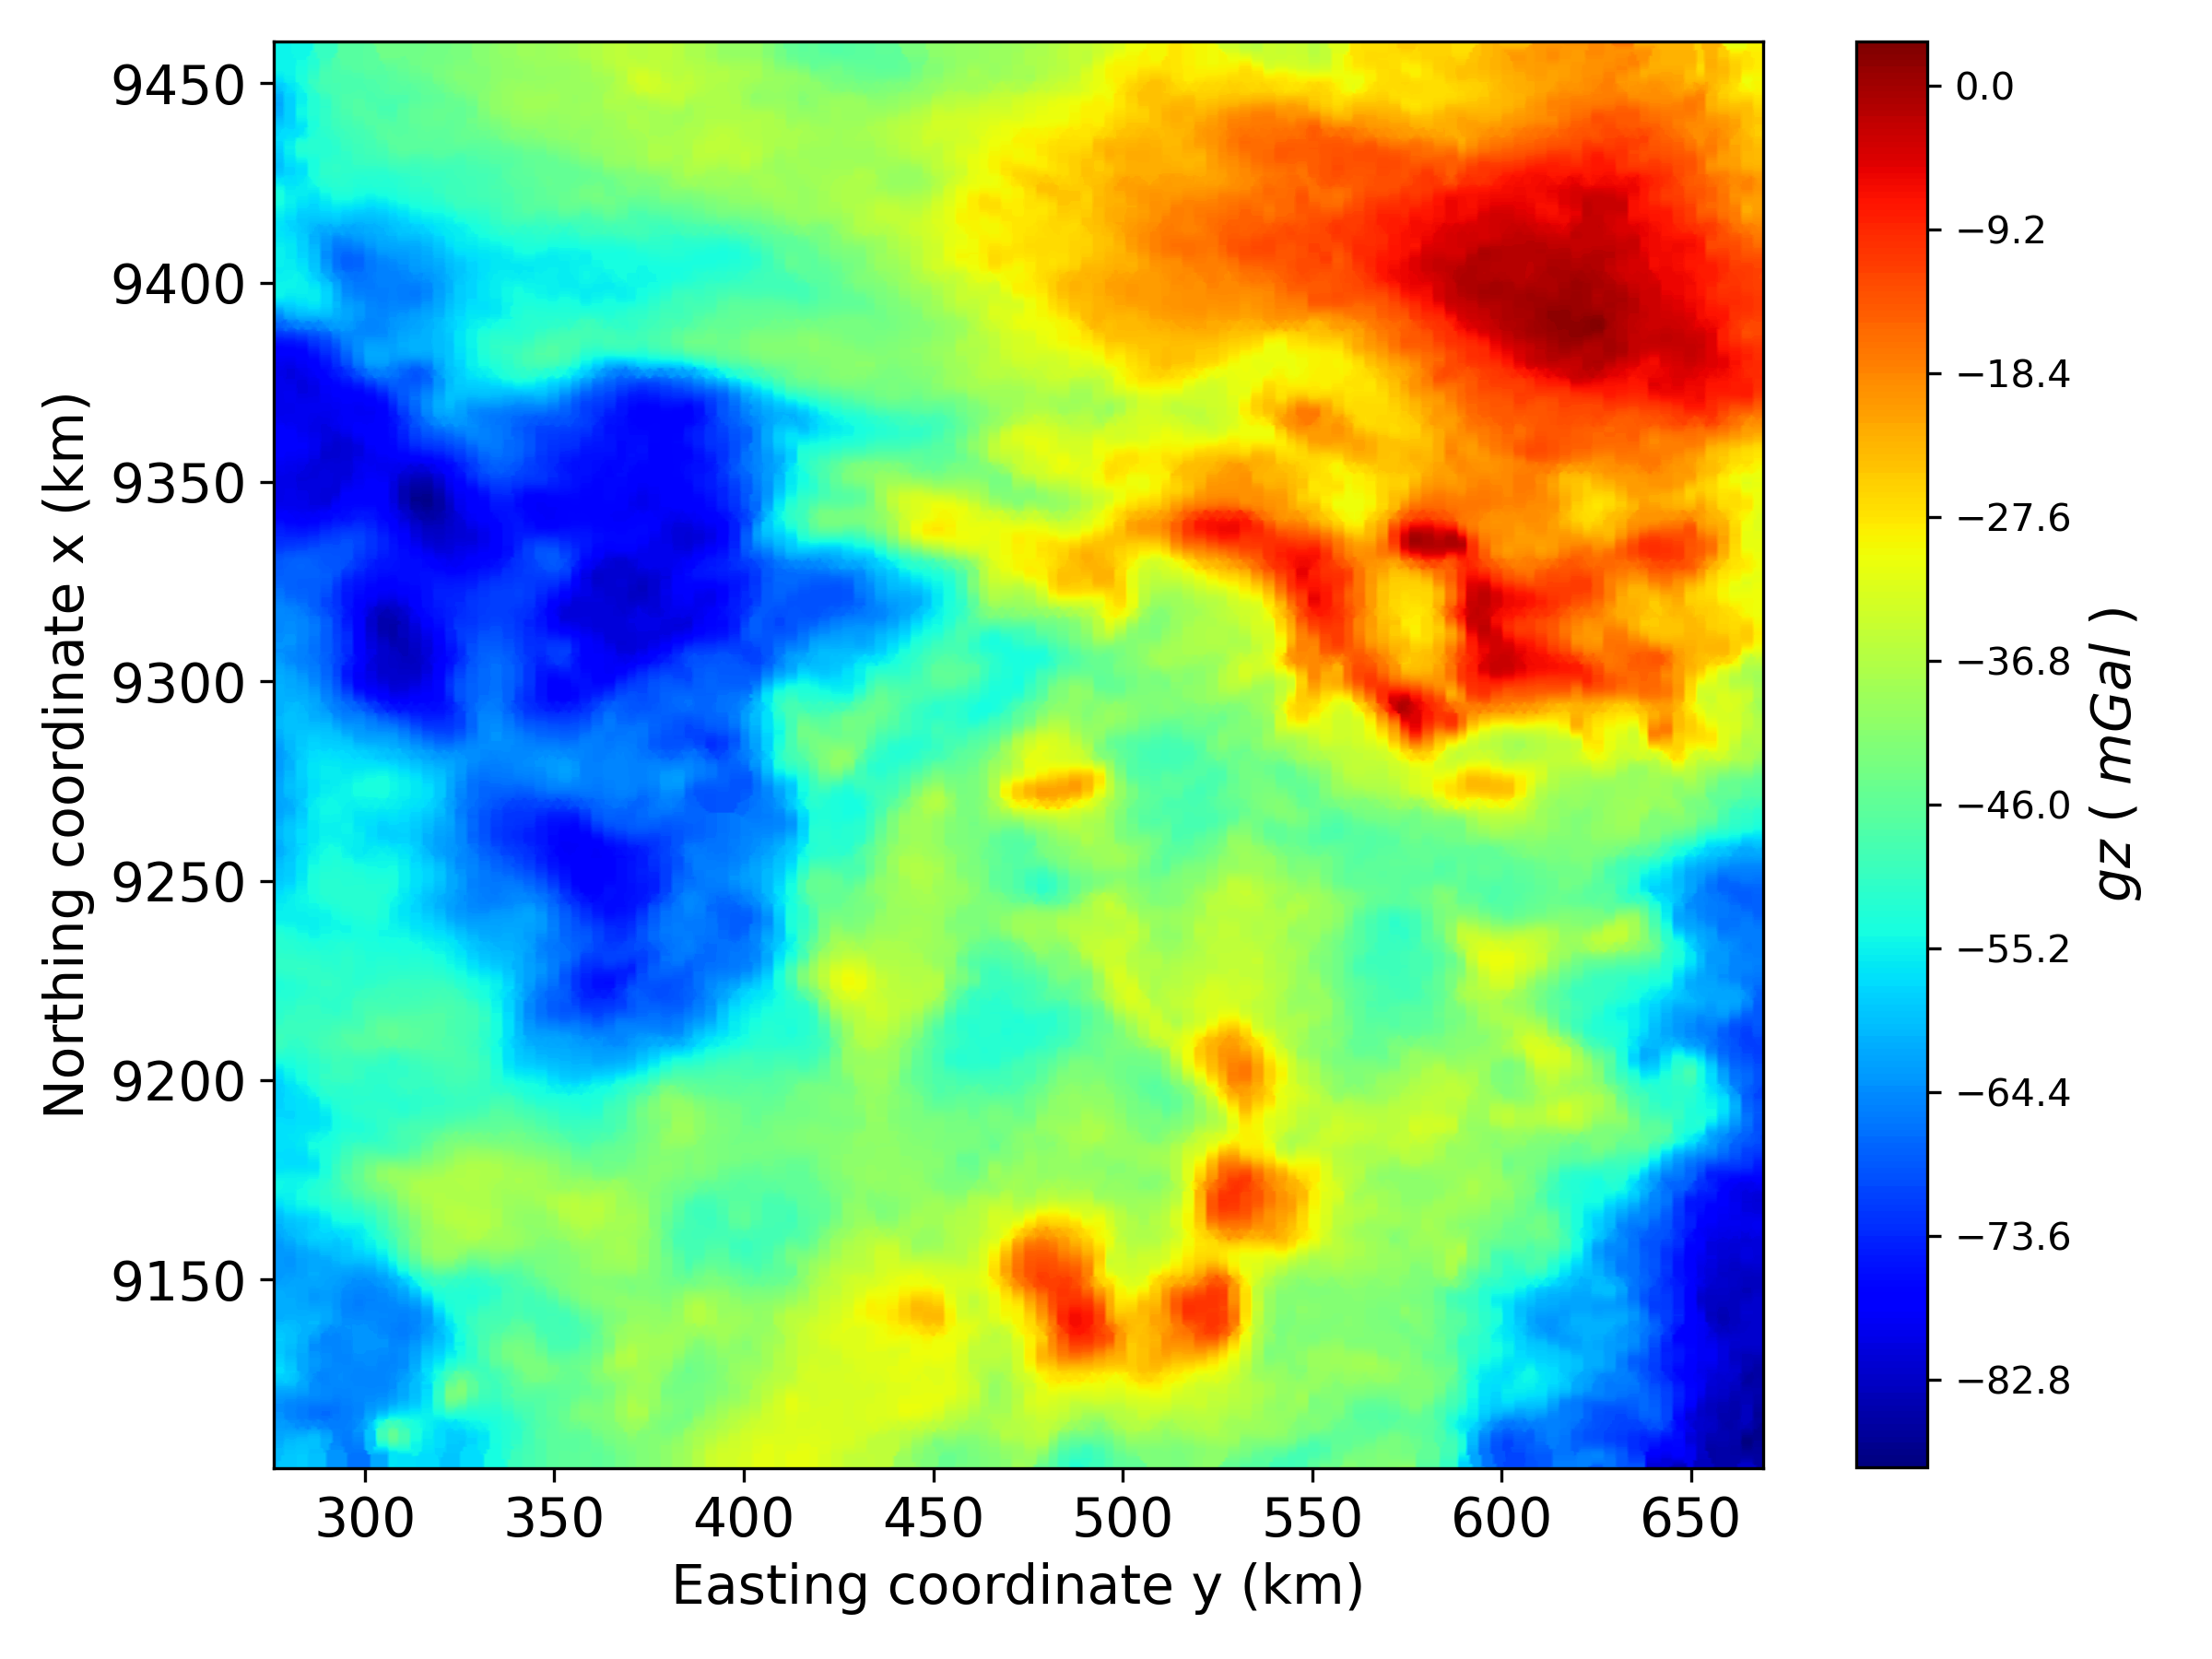
\includegraphics[width=10cm]{Fig/carajas_gz_real_data_1000x500}
	\end{center}
	\caption{
		Field aerogravimetric data over Caraj{\'a}s, Brazil. 
		There are $D = 500, 000$ observations located on regular grid of $1,000 \times 500$ poins.
		}
	\label{fig:9}
\end{figure}

\begin{figure}[htbp]
	\begin{center}
		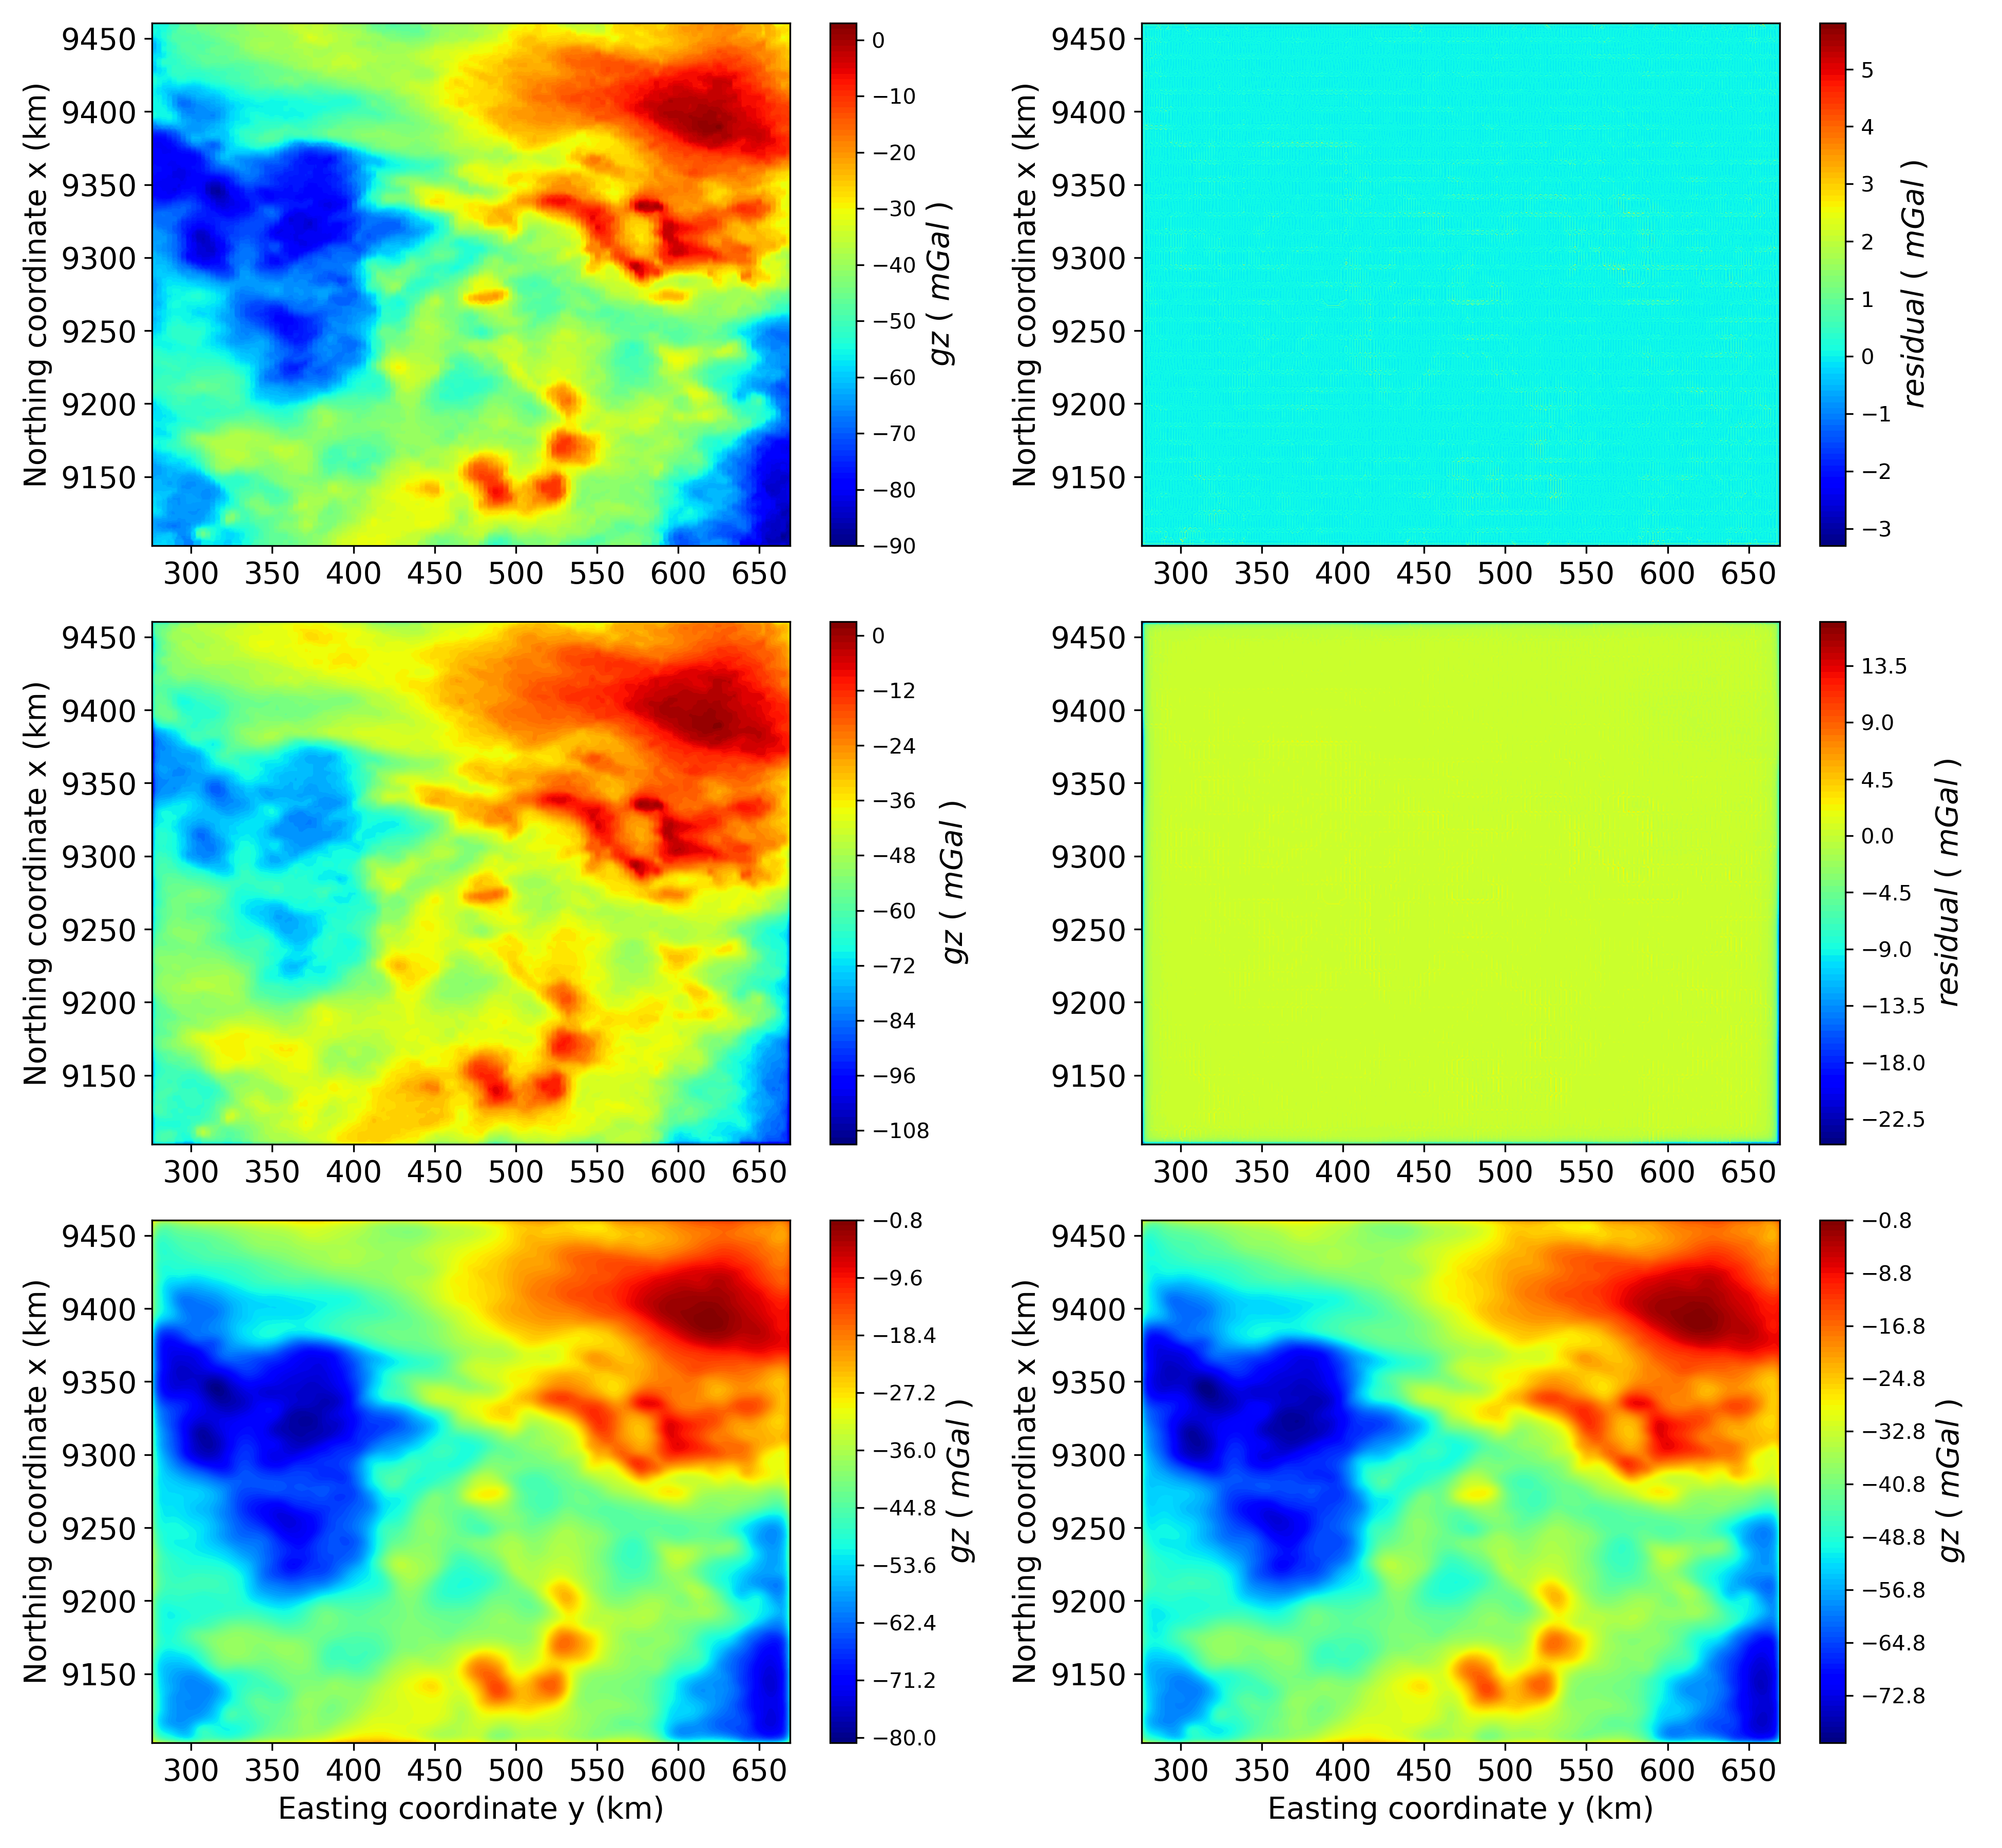
\includegraphics[width=10cm]{Fig/carajas_gz_predito_1000x500}
	\end{center}
	\caption{
		Upward continuation of the aerogravimetric data over Caraj{\'a}s, Brazil.
		\textbf{(A)} Predicted data due to the equivalent layer obtained from the iterative deconvolution 
		(Algorithm \ref{alg:TOB20-22}) with $50$ iterations.
		\textbf{(B)} Residuals between the predicted data shown in \textbf{(A)} and the observed data (Figure \ref{fig:9}). 
		\textbf{(C)} Predicted data due to the equivalent layer obtained from the direct deconvolution computed with $\zeta = 10^{-22}$
		(equation \ref{eq:matrix-L-Wiener-deconvolution}). 
		\textbf{(D)} Residuals between the predicted data shown in \textbf{(C)} and the observed data (Figure \ref{fig:9}). 
		\textbf{(E)} and \textbf{(F)} Continued field at $z = -3500 \mathrm{m}$ obtained from iterative and direct deconvolutions.
		}
	\label{fig:10}
\end{figure}

\begin{figure}[htbp]
	\begin{center}
		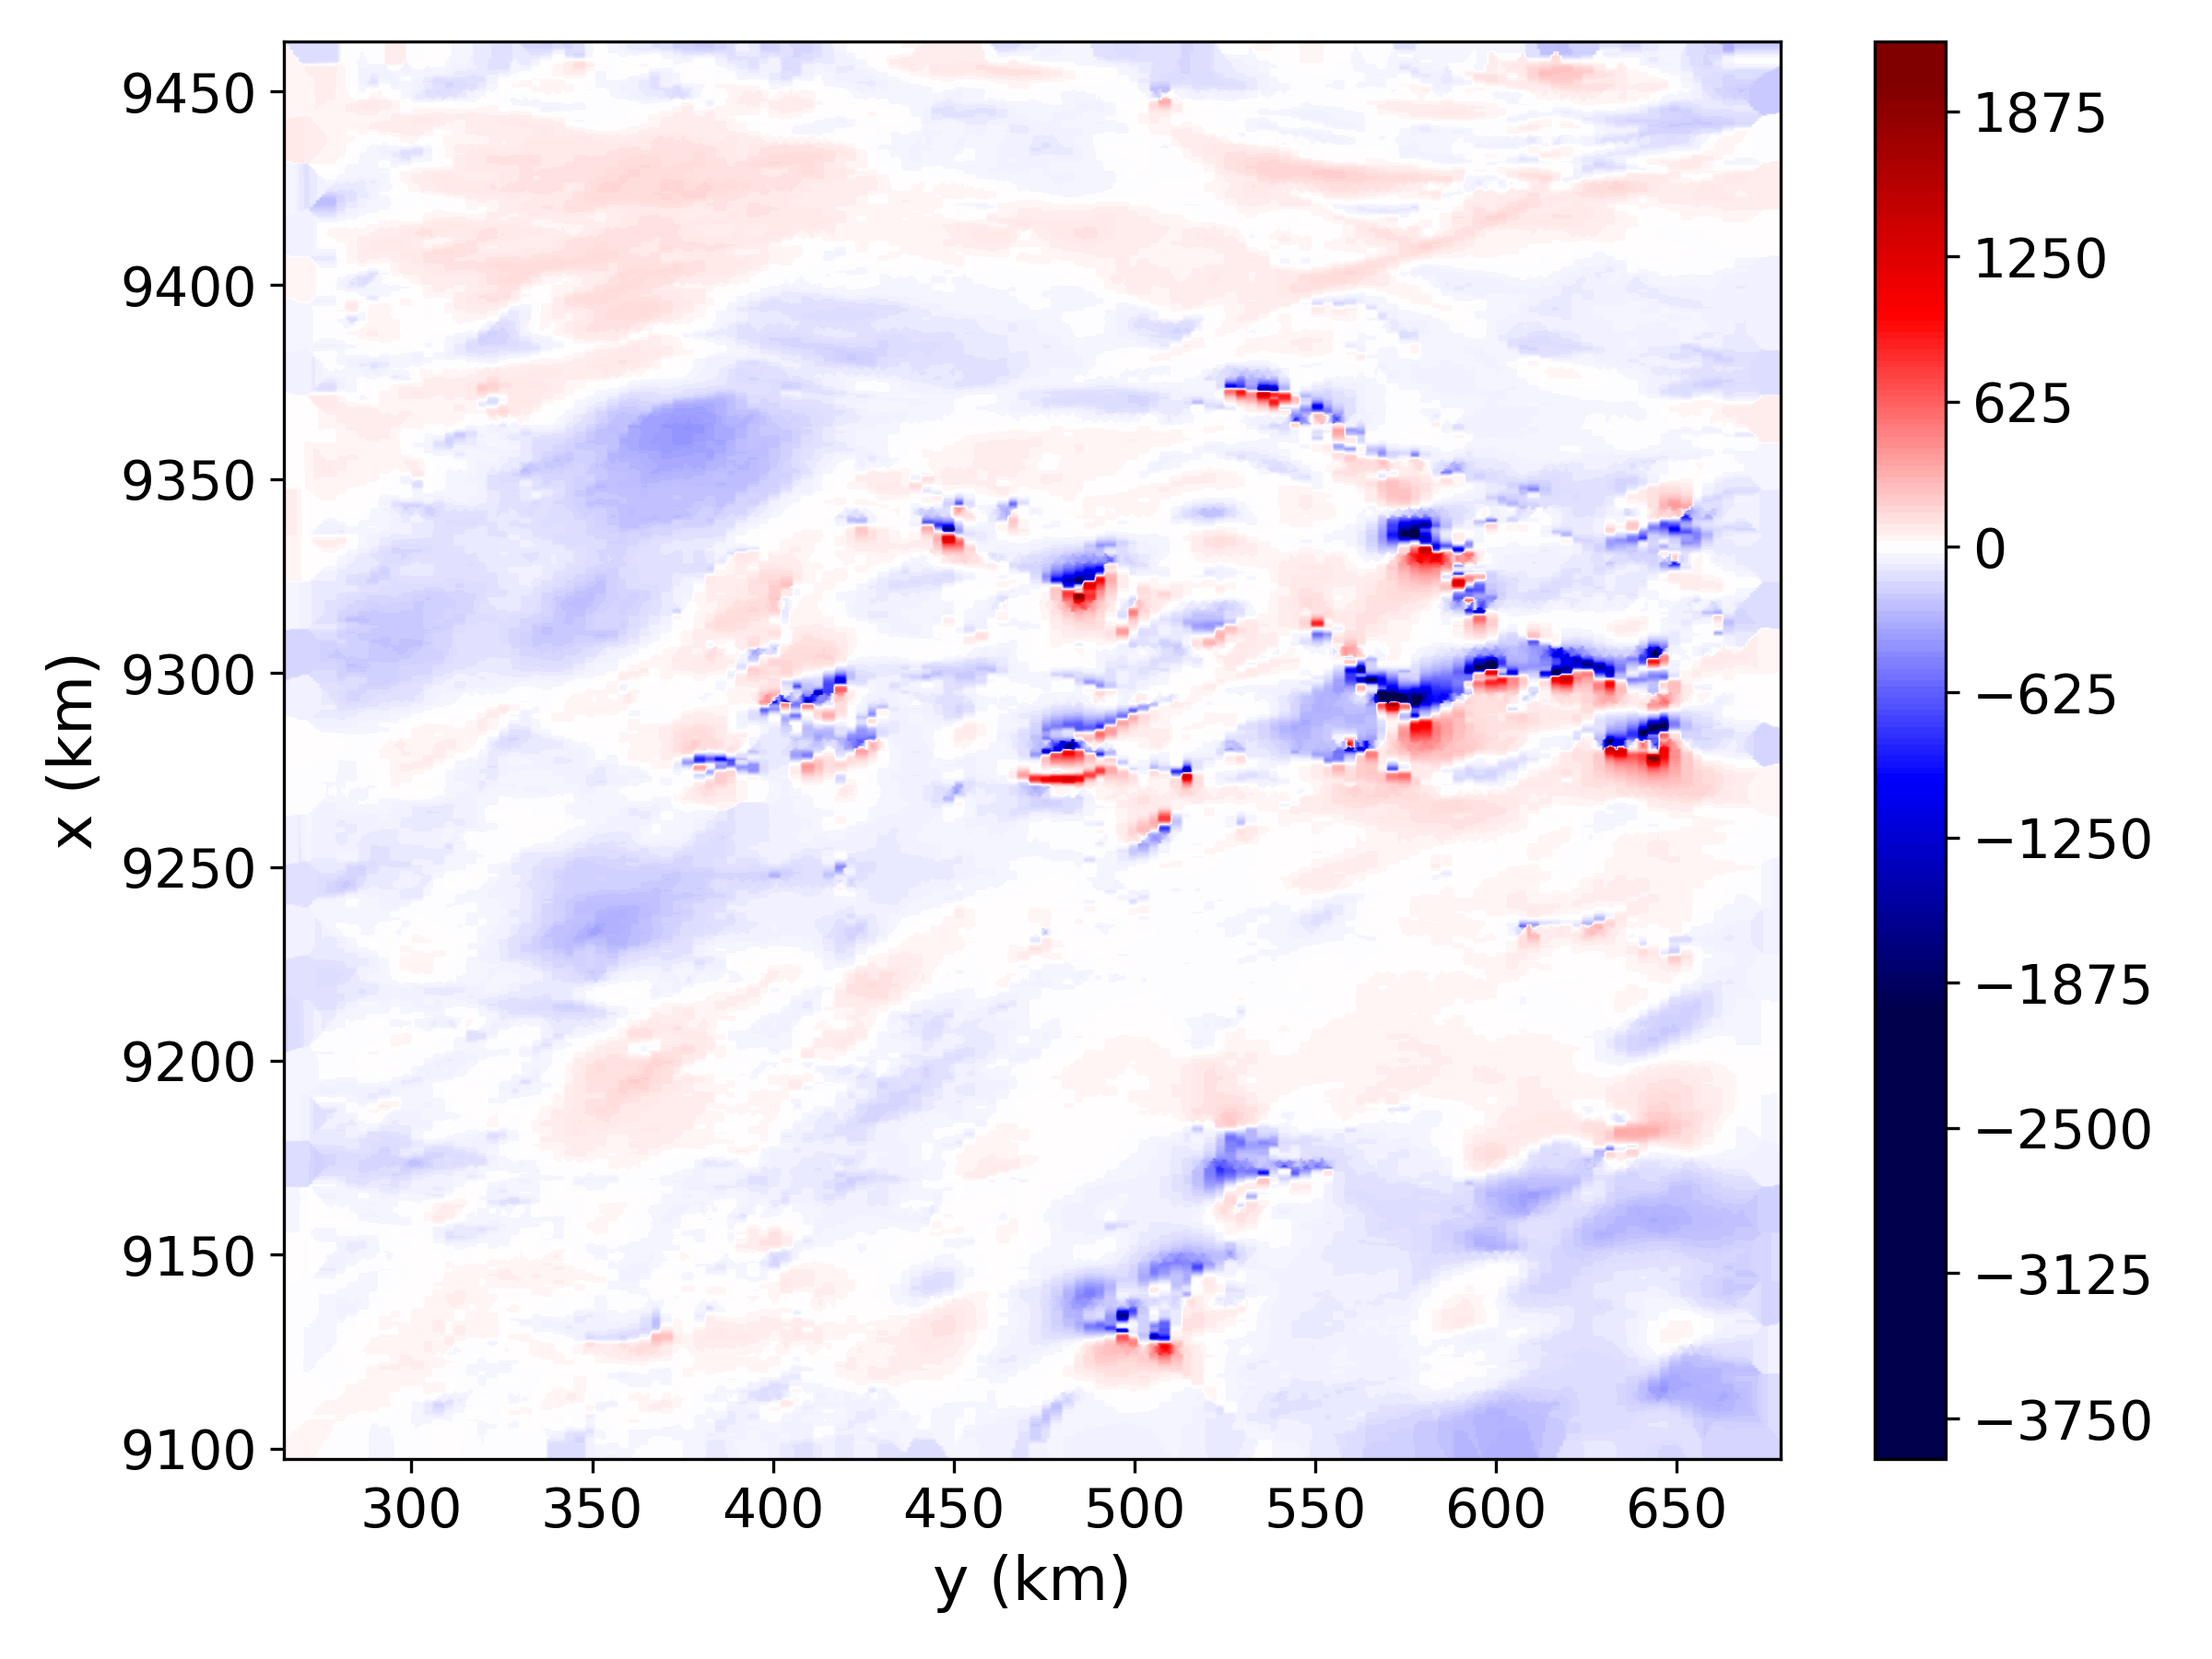
\includegraphics[width=10cm]{Fig/carajas_tf_real_data_1000x500}
	\end{center}
	\caption{
		Field aeromagnetic data over Caraj{\'a}s, Brazil. 
		There are $D = 500, 000$ observations located on regular grid of $1,000 \times 500$ poins.
		}
	\label{fig:11}
\end{figure}

\begin{figure}[htbp]
	\begin{center}
		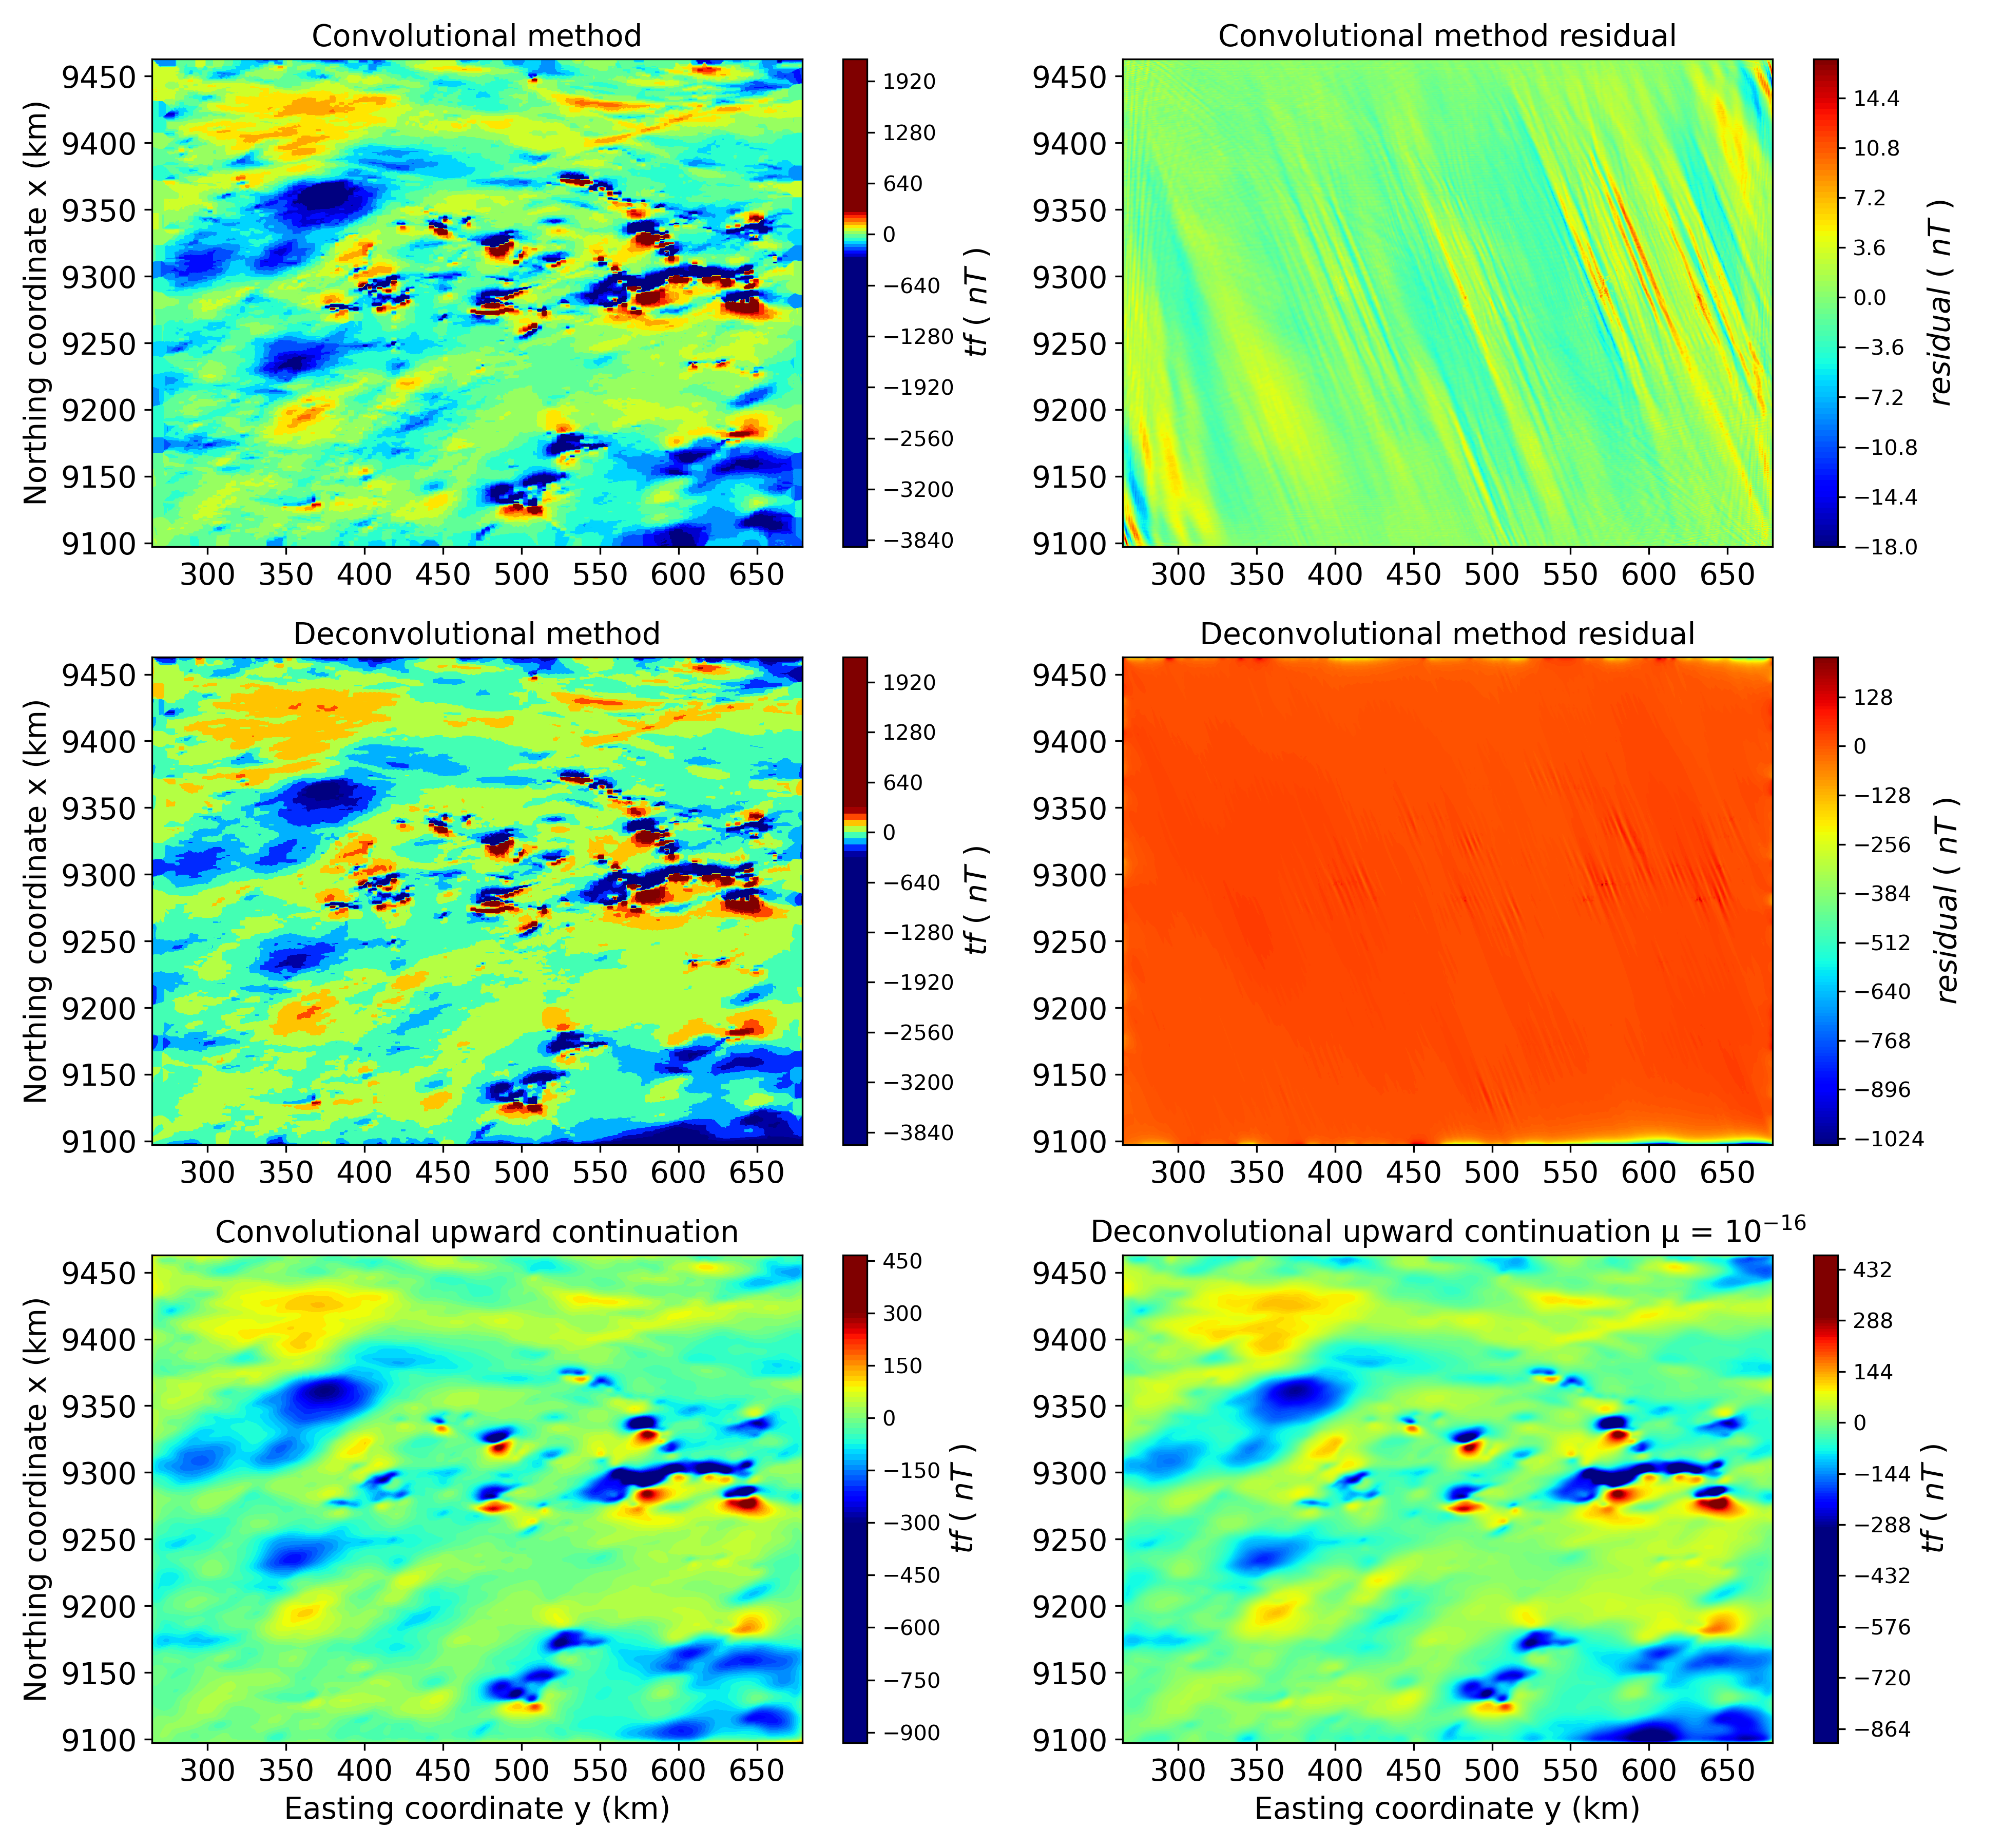
\includegraphics[width=10cm]{Fig/carajas_tf_predito_1000x500}
	\end{center}
	\caption{
		Upward continuation of the aeromagnetic data over Caraj{\'a}s, Brazil.
		\textbf{(A)} Predicted data due to the equivalent layer obtained from the iterative deconvolution 
		(Algorithm \ref{alg:TOB20-22}) with $200$ iterations.
		\textbf{(B)} Residuals between the predicted data shown in \textbf{(A)} and the observed data (Figure \ref{fig:11}). 
		\textbf{(C)} Predicted data due to the equivalent layer obtained from the direct deconvolution computed with $\zeta = 10^{-16}$
		(equation \ref{eq:matrix-L-Wiener-deconvolution}). 
		\textbf{(D)} Residuals between the predicted data shown in \textbf{(C)} and the observed data (Figure \ref{fig:11}). 
		\textbf{(E)} and \textbf{(F)} Continued field at $z = -3500 \mathrm{m}$ obtained from iterative and direct deconvolutions.
		}
	\label{fig:12}
\end{figure}

%%% If you are submitting a figure with subfigures please combine these into one image file with part labels integrated.
%%% If you don't add the figures in the LaTeX files, please upload them when submitting the article.
%%% Frontiers will add the figures at the end of the provisional pdf automatically
%%% The use of LaTeX coding to draw Diagrams/Figures/Structures should be avoided. They should be external callouts including graphics.


%\bibliographystyle{frontiersinSCNS_ENG_HUMS} %  for Science, Engineering and Humanities and Social Sciences articles, for Humanities and Social Sciences articles please include page numbers in the in-text citations
%\bibliographystyle{frontiersinHLTH&FPHY} % for Health and Physics articles
%\bibliography{test}

%\end{document}
